\documentclass[a4paper,12pt]{article}
\usepackage[utf8]{inputenc}
\usepackage{graphicx}
\usepackage{supertabular}
\usepackage[draft]{fixme} % \fxnote  \fxwarning  \fxerror  \fxfatal
\usepackage{subfigure}
\usepackage[final]{pdfpages} %To add the pdf page as frontpage
\usepackage{booktabs} %For tables, horizontal and splittable lines
\usepackage{rotating}
\usepackage[format=hang,font=small,labelfont=bf]{caption} %To create bold caption for tables and pictures
\setcounter{secnumdepth}{3} %Chap,Sec,Sub,Subsub
\usepackage{fullpage} % to use the whole page 
\usepackage{url}
\usepackage{setspace}  
\usepackage{hvfloat}
\usepackage{multicol}
\usepackage{xcolor}
\usepackage{listings}
\doublespacing     % Inter lines space

%%%%%%%%%%%%%%% FANCY HDR Settings %%%%%%%%%%%%%%%%%%%%%%%%%%%%%%%%%%%%%%%%%%%
\usepackage{fancyhdr}
%\usepackage[head=30pt,foot=10pt]{geometry}
%\fancypagestyle{plain}
\pagestyle{fancy}
\setlength{\headheight}{15pt} %Set the height of the header
\topmargin=-20pt
\headsep = 35pt
\hoffset=+0.335in
\textwidth = 445pt
%\footheight = 10pt
\textheight = 680pt %715

\fancyheadoffset[L]{35pt} % gap between the header and the left side 
\fancyheadoffset[R]{10pt} % gap between the header and the left side 
%\fancyfootoffset[R]{10pt}
\footskip = 30pt
%\voffset=-3.5in

\fancyhead{} %Clear all headers
\fancyhead[R]{\slshape \rightmark} % To write the Subsection on the upper right[R] header side
%\fancyhead[LO]{\slshape \leftmark} % To write the Section on the upper Left header side
%\fancyhead[R]{\bfseries Enabling BPEL service execution on Java devices by means of model-to-text transformations} %To write the Thesis title on the upper Right header

\lhead{\setlength{\unitlength}{1mm}
\begin{picture}(0,0)
\put(0,0){
\includegraphics[width=65mm]{pictures/Logo.png}}
\end{picture}}

\fancyfoot{} %Clear the footer
\fancyfoot[C]{\slshape \thepage}

%%%%%%%%%%%%%%%%%%%%%%%%%%%%%%%%%%%%%%%%%%%%%%%%%%%%%%%%%%%%
%%%%%%%%%%%%LST listings settings %%%%%%%%%%%%%%%%%%%%%%%%%%

% Basic settings of the listings package to "better" show the code 

% \lstset{ %
% language=Java,            % choose the language of the code
% basicstyle=\small,  % the size of the fonts that are used for the code
% basewidth={0.57em,0.57em},
% %frame=trBL,			        % adds a frame around the code
% breaklines=true,		      % sets automatic line breaking
% showstringspaces=false,         % underline spaces within strings
% }
%%%%%%%%%%%%%% LSTLISTINGS SETTINGS, creation of schema colors for BPEL/XML/ACCELEO and JAVA %%%%%%%%%%%%%%%%%%%%%
%%%%%%% BPEL - XML - ACCELEO
\definecolor{lightgray}{RGB}{10,40,40}
\definecolor{darkgray}{rgb}{.4,.4,.4}
\definecolor{forestGreen}{RGB}{34,139,34}
\definecolor{orangeRed}{RGB}{255,69,0}

\lstdefinelanguage{bpel}{
morekeywords=
{name,linkName,isolated,parallel,partnerLink,operation,portType,inputVariable,createInstance,variable,element,location,importType,partnerLinkType,myRole,messageType,properties,level,outputVariable,xmlns,version,encoding}
}

\lstdefinelanguage{acceleo}{
morekeywords=
{template,query,comment,for,if,file,let,protected,super,module}
}

\lstdefinelanguage{xml}{
        basicstyle=\footnotesize,
        sensitive=false,
}        

\lstdefinestyle{workflowStyle}{
language=XML,
alsolanguage=bpel,
alsolanguage=acceleo,
%Formatting
basicstyle=\footnotesize,
sensitive=true,
showstringspaces=false,
numbers=left,
numberstyle=\scriptsize,
tabsize=4,
numbersep=3pt,
extendedchars=true,
xleftmargin=2em,
lineskip=1pt,
breaklines,
captionpos=t,
%Coloring
backgroundcolor=\color{blue!8!white},
morekeywords={BooleanExpression},
alsoletter={:,<,>,/,?},
morestring=[b]{"},
morecomment=[s]{<!--}{-->},keywordstyle=\color{forestGreen},
identifierstyle=\color{blue}\ttfamily,
stringstyle=\color{orangeRed}\ttfamily,
commentstyle=\color{forestGreen}\ttfamily
}
% new environment for xml/BPEL/Acceleo
\lstnewenvironment{workflow-code}[2]{
\lstset{caption=#1,label=#2,style=workflowStyle}
}{}
%%%%%%%% Java lstlisting settings
\definecolor{javared}{rgb}{0.6,0,0} % for strings
\definecolor{javagreen}{rgb}{0.25,0.5,0.35} % comments
\definecolor{javapurple}{rgb}{0.5,0,0.35} % keywords
\definecolor{javadocblue}{rgb}{0.25,0.35,0.75} % javadoc
% no need to redefine the constructs list, they are already defined in lstListing
\lstdefinestyle{javaStyle}{
language=Java,
%Formatting
basicstyle=\footnotesize,
sensitive=true,
showstringspaces=false,
numbers=left,
numberstyle=\scriptsize,
tabsize=4,
numbersep=3pt,
extendedchars=true,
xleftmargin=2em,
lineskip=1pt,
breaklines,
captionpos=t,
%Coloring
backgroundcolor=\color{blue!8!white},
keywordstyle=\color{javapurple}\bfseries,
stringstyle=\color{javared},
commentstyle=\color{javagreen},
morecomment=[l][\color{javadocblue}]{//},%,
}
% new environment for Java
\lstnewenvironment{java-code}[2]{
\lstset{caption=#1,label=#2,style=javaStyle}
}{}
%%%%%%%%%%%%%%%%%%%%%%%%%%%%%%%%%%%%%%%%%%%%%%%%%%%%%%%%%%%%

% Last package to be imported
\usepackage[pdftex,linkbordercolor={0 0 1},bookmarks=true,hypertexnames=false,breaklinks=true]{hyperref}
\hypersetup{
pdfauthor = {Antonio Arfè},
pdftitle = {Enabling BPEL service execution on Java devices by means of model-to-text transformations},
pdfcreator = {LaTeX},
pdfproducer = {latex + ps2pdf}}

% Title Page
\title{Enabling BPEL service execution on Java devices by means of model-to-text transformations}
\author{Antonio Arf\`{e}}

% Commands for showing the most used acronyms
\newcommand{\nl}{\newline} 
\newcommand{\javarmi}{\textsc{Java RMI}}
\newcommand{\bpel}{\textsc{BPEL}}

% Make every section start in a new page
\let\stdsection\section  
\newcommand{\STE}[1]{\textcolor{red}{#1}}
\renewcommand\section{\newpage\stdsection}

%%%%%%%%%%%%%%%%%%%%%%%%%%%%%%% END SETTINGS %%%%%%%%%%%%%%%%%%
%%%%%%%%%%%%%%%%%%%%%%%%%%%%%%% BEGIN DOCUMENT %%%%%%%%%%%%%%%%

\begin{document}

% % % \thispagestyle{empty}
% % %  \begin{titlepage}
% % %  % - Begin of frontpage -
% % %  \fxnote{DRAFT version 1.0}
% % %  \begin{nopagebreak}
% % % 
% % % \begin{raggedleft}\advance\rightskip by-1cm
% % % \null\vskip 2.5cm
% % %      {\LARGE Antonio Arfè}
% % % \vskip 2cm
% % % {\fontsize{28}{32}\bfseries
% % % Enabling BPEL service execution on Java devices by means of model-to-text transformations fixme
% % % 
% % %  \par}
% % % \vskip 3cm
% % % {\Large Bachelor Thesis Project \ June 2012 - ---- 2012 \par} %fixme
% % % \vskip 3pt
% % % To be evaluated on fixme --$^{th}$ 2012  %fixme
% % % \end{raggedleft}
% % % \vfill
% % % \hbox{\vrule\vbox{\hrule
% % %                 \prevdepth0pt
% % %                 \vskip2pt
% % %                 \hbox{ Department of Computer Science }
% % %                 \hbox{ Federico II University}
% % %                 \hbox{ Via Claudio,}
% % %                 \hbox{ 80100 Naples }
% % %                 \hbox{ ITALY }
% % %                 \vskip2pt
% % %                 \vskip.5ex
% % %                 \vskip2pt
% % %                 \hrule}\vrule}
% % % 
% % %  \end{nopagebreak}
% % % 
% % %  \cleardoublepage
% % %  
% % % % - End of frontpage - begin of titlepage -
% % % \begin{nopagebreak}
% % % {\samepage
% % % \begin{tabular}{lr}
% % %         \parbox{14.5cm}{
% % %           {\LARGE Faculty of Engineering}
% % % 
% % %           {\small Federico II University}
% % %           \vspace{-0.3cm}\\
% % %         \hrule
% % %         \vspace{0.2cm}
% % %           {\bf Department of Computer Science}
% % %          }   & \hspace{-2.0cm} %
\includegraphics[width=1.1cm]{picLogo.jpg} %fixme
% % % \end{tabular}
% % % %------------------------ with parbox at 7 cm
% % % \begin{tabular}{cc}
% % % \parbox{7cm}{
% % % \hspace{2cm}
% % % \begin{description}
% % % 
% % % \item {\bf TITLE:}
% % % 
% % % Enabling BPEL service execution on Java devices by means of model-to-text transformations
% % % 
% % % \end{description}
% % % 
% % % % ---------------------- Description with parbox at 8 cm
% % % \parbox{8cm}{
% % % 
% % % \begin{description}
% % %          \item {\bf PROJECT PERIOD:}\\
% % %            Bachelor Thesis, \\
% % %            %fixme Oct 1$^{st}$ 2012 -\\fixme 99$^{th}$ 2010\\
% % %             June 2012 -\\---- 2012\\
% % %            \hspace{4cm}
% % %          \item {\bf STUDENT:}\\
% % %            Antonio Arfè\\
% % %            \hspace{2cm}
% % %          \item {\bf SUPERVISORS:}\\
% % %            V. Vittorini, S. Marrone
% % % \end{description}
% % % }
% % % 
% % % %--------------------------------------------------------
% % % \begin{description}
% % %         \item {\bf NUMBER OF COPIES:} 4
% % %         \item {\bf REPORT PAGES:} \pageref{report_end}
% % %         \item {\bf APPENDIX PAGES:} 0
% % %         \item {\bf TOTAL PAGES:} \pageref{LastPage}
% % % \end{description}
% % % %--------------------------------------------------------
% % % \vfill } &
% % % \parbox{7cm}{
% % %   \vspace{.15cm}
% % %   \flushright
% % %   \fbox{
% % %     \parbox{6.5cm}{{\bf SYNOPSIS:}\vspace{0.5cm}
% % %      {\vfill{\small % Synopsis


	fixme.

	Lorem ipsum dolor sit amet, consectetur adipiscing elit. Sed lorem ante, porttitor vitae fringilla et, fermentum fermentum nisl. Nunc fringilla, dui viverra iaculis volutpat, augue massa ornare augue, ac sodales erat lectus non risus. Cras rutrum elit sit amet ligula interdum fermentum. Curabitur tincidunt, dui ut hendrerit mattis, massa turpis pretium lectus, eu sagittis turpis nibh id sem. Vestibulum consectetur sapien vel nisi vehicula eget dignissim diam malesuada. Cras consequat, tellus ut malesuada commodo, lacus libero adipiscing ligula, auctor laoreet ligula enim eu turpis. Aenean eget dui eget mauris facilisis faucibus. Curabitur quis metus est, a vulputate orci. Integer mollis metus ac purus condimentum

	fixme.
% % %      }}\vspace{0.3cm}
% % %      }
% % %   }
% % % }
% % % \end{tabular}
% % % }
% % % 
% % % %----------------------
% % % 
% % % \end{nopagebreak}
% % % \end{titlepage}

 
%\setcounter{page}{3}

\includepdf[pages=1-2]{frontespizio.pdf}
%pagina vuota se possibile

% Table of contents
\tableofcontents
\pagebreak

\section{Introduction}
%---Web Services Composition Contest

Today the web is quickly expanding and new functionalities and applications, appearing day by day, are heavily increasing its potentialities and ease of use. Actually, one of the reasons why this growth is taking place is the possibility to connect and let communicate different existent applications, or better, \textit{services}. Now more than ever, with the wide expansion of portable and web-capable devices, based on different technologies, platforms or hardware, this interconnection among services is not only required, but necessary to create a common ground to build software upon.\\

The interconnection among services can be done through ad-hoc solutions, for example, connecting some preexistent legacy applications to create a new application (perhaps available online or over a company's intranet) or using standard paradigms to wrap existing applications and publish them as services. %SOC 
In the case where the standard paradigm is favored, the implementation of such services also needs an architectural infrastructure style. This architecture precisely defines the three main roles: which part of the application is offering the service to the outside world (Service Provider), where the service should be published for a public usage (Service Registry) and who is the user of the service (Service Client). %SOA
A service implemented following such an architecture and guidelines, where its communication channel is the web, is called \textit{Web Service}.\\ %(cite intoduzione ragionata al mondo dei web serv)

Once, starting from simple applications, several services are put in place, to reach the goal of creating a new application (which can be, recursively, used as basic service to create another application) reusing the existing ones, many challenges arise. Some of them are: how to discover the services that are publicly available, how the providers can advertise them, how the services should integrate the usage of resources like files or databases, how they provide secure and private access to authorized users and, eventually, how to define the rules to compose and make collaborate the services together. 
The final result of the interactions among the different services is called \textit{Business Process}, which is widely used in the literature and compares in the acronym of some of the main languages used in the service-oriented applications area.\\

Focusing on the latter aspect, the composition of services, it can be achieved using workflow management applications, that simultaneously coordinate different processes, making them execute actions in sequence or in parallel, and joining or forking their results at the right time. %(Intro Ragionata WS)
The two main approaches to workflow management are: Orchestration and Choreography.
Orchestration refers to the %(cite introduzione ragionata al mondo dei web serv, pag 20) 
business process realized by the interaction of several services supervised by a main actor. Choreography, instead, is a more collaborative approach, where each of the services has a specific role in the accomplishment of the business process. Eventually, orchestration produces an executable process, which can be run by an orchestration engine, while choreography produces an abstract business protocol that cannot be executed, but only contains the specification of the publicly available messages exchanged between the services.

\paragraph{The problem}
Today, many of these services, which can be later interconnected, need to run on portable devices, for which calculation power, available memory and consumption are well known issues. In fact, the composition and orchestration (or choreography) of a business process is heavy, and the majority of workflow engines are made to be run on powerful machines both in terms of computation and memory footprint. Moreover the deployment of a business process usually requires to know a priori the number of participant devices, and, above all, it requires them to have installed network protocols and tools that are not always included in the typical software package of a mobile device. 
Nonetheless, many business processes are already available written in the de facto standard language for web services orchestration: BPEL (Business Process Execution Language). Although there have been attempts to create light and with low memory footprint engines (\cite{bpelMobileEngineMora,bpelMobileEngineHackmann06sliver:a}), the execution of a BPEL process on a small, portable device, is yet to be convenient.

In opposition, in the last years, other technologies have widely spread and have been optimized for the mobile devices world. One as such is surely Java, which has gained ground thanks to its portability, which completely abstracts the software from the hardware. This makes it easy for software companies to produce reusable software, independently of the device architecture. Moreover,the Java relatively ease of use, the large amount of available libraries and the large user community, surely also play in its favour. 
%There are other approaches used to compose and coordinate services (namely, to create a business process), there are RPC and JAVA RMI.

\paragraph{Objective}
Given the widespread presence over the web of BPEL for service-oriented applications implementation, we analyze the possibility of automatically transform a BPEL written process in a Java executable routine, with minimum ad-hoc developer's intervention.
Our objective is then to show the feasibility of a semi-automated transformation from a small business process orchestrated with BPEL to the well known and wide spread over mobile devices, Java language. 


%---Other works, our approach and what we achieve
%\subsection{Other works}
% - Other similar works: don't know any yet. \nl
% - Our attempt is to use the M2T techniques to obtain from a BPEL WSs composition a JavaRMI equivalent application \nl
% - Where the limits of our solution are (BPEL subset? Lack of heavy test case? Doesn't work at all?...) \nl
% - Where future work might be leaded \nl



%---Overview of the whole work---
\subsection{Overview of the thesis}
FIXME : To expand at the end

%  \item Proposed approach, MDE, MDA
% \end{itemize}


%Generic stuff
% We intend the word \textit{service} as the one used by the UDDI Oasis consortium \cite{Uddi}, where services are self-contained and modular applications that have Internet-oriented and standard-based interfaces. The given definition of services tightly relates to some of the well known web standards used to implement Web Services (WSs) \cite{DiLorenzo08}.
%Service Oriented Computing
\section{Service Oriented Computing}
\label{ServiceOrientedComputing}
This Section gives a brief overview of the Service Oriented domain and its components. We introduce in Section \ref{SOC&SOA} the paradigms to create service oriented infrastructures. Section \ref{WebServices} explains how services can be deployed using the web as media, namely, the Web Services. 
Later in Section \ref{WFManagement} we talk about Workflow management, introducing the terms of Orchestration and Choreography. Right after we dig into the technologies we will be working on throughout the whole project; we overview both BPEL in Section \ref{BPEL} and the remote calls enabled version of Java, Java RMI in Section \ref{JavaRMI}.   

\subsection{Services and composition, SOC and SOA}
\label{SOC&SOA}
During the years preceding the large spread of the Internet, companies used to create their own software systems, in order to obtain highly customized and specific services, rarely focused on the accessibility by external partners.
Today, with the necessity of exchanging information among different companies and businesses, and the push made by the large growth of the Internet, the focus has moved to the integration and the coordination of the existing softwares, namely, the integration of these systems over larger networks.
Defining a \textit{service} as a distributed application that exports a view of its functionalities  \cite{DiLorenzo08}, what is needed is the possibility to compose different services together.
For example, it might be useful to integrate a service (already available on a net), providing maps of a city's streets, with a web-based service listings telephone numbers of a given city zone, resulting in a new service showing telephone numbers on the map. %\fxnote{I might add a picture to better show the example here} FIXME
  
The \textit{Service Oriented Computing} (SOC) is the paradigm that attempts to wrap and adapt existing applications into new services, which should comply to three main requirements \cite{DiLorenzo08,Papazoglou03}:
\begin{itemize}
 \item technological independent: the service should be accessible via well known protocols and have a descriptions available on most of the IT environments.
 \item loosely coupled: the client and the provider of the service should not know each other's internal details.
 \item location transparent: clients should be able to get information and access to a service, irrespectively of their location. 
\end{itemize}
Eventually the SOC paradigm makes use of services as the atomic components for developing new applications (which, in turn, can be services too \cite{Papazoglou03}.


To apply the SOC paradigm, there is a need of an architecture infrastructure style, which gives the directives and guidelines to build such a service.  
The architectural infrastructure of the SOC is called \textit{Service Oriented Architecture} (SOA). 
The idea behind the SOA is to describe, publish and make available services (generally speaking, a combination of services) obtained from a preexistent set of applications. 
To achieve the results of making non-homogeneous applications, using different technologies and running on different platforms, work together, SOA makes use of standard interfaces and messaging protocols. This way each of the applications become an atomic, well defined and ready to be connected component. 
The SOA presents an architecture devised in three main components \cite{Pernici04}:
\begin{itemize}
 \item Service provider
 \item Service registry
 \item Service client
\end{itemize}
%as shown in Fig. FIXME: toCreate\ref{fig:The Service Oriented Architecture (SOA)}:
A \textit{service provider}, which makes the service available. The service provider registers its service to the \textit{service registry}, which contains the list of available services and their descriptions. After the registration, the service provider waits for a client to request a service. The service registry can also apply custom access control policies or be entirely public. 
The \textit{service client} contacts the service registry to \textit{find} a service, it gets a contract and the address of the service, making a so called \textit{bind} with the provider. Then it \textit{uses} the service.


Being the realization of services usually based on the reuse of previously existent software, there are many ways to realize it and they can also be combined. For a company, the realization can go from the complete in-house realization to the outsourcing, to buy/leasing just parts of the needed services or to using wrappers/adapters to reuse the legacy software.
To conclude, from the SOA point of view, services are like black boxes, they can be invoked by service clients independently, without the need of knowing internal details. This makes clients and providers logically decoupled, the client only needs to know the name, the interface and the version of the service. Of course, provider, client and register must be able to use a common communication channel. 

\subsection{Web Services}
\label{WebServices}
We have seen that SOA is an architecture style aimed at the creation of services but it does not address the communication medium. \textit{Web Services} (WS) are an instance of a SOA where the communication channel is the web \cite{Pernici04}.
Web services implement the SOA through the application of three main technologies: \textit{SOAP}(Simple Object Access Protocol), \textit{WSDL}(Web Services Description Language) and \textit{UDDI}(Universal Description, Discovery and Integration).
On the picture of the SOA showed above, we can add these three components.
%, as shown in Fig: (FIXME: to create)\ref{fig:SOA with webServ implement.}.
The SOAP is the web protocol used to exchange messages among the parties. WSDL is the language used by the service provider to fully describe the offered service. At last, UDDI is used by the service registry to make a service easy to find, abstract its technology and make it accessible to the clients.
In the next paragraphs we have a brief look into these three technologies.

\subsubsection{WSDL (Web Services Description Language) }
\label{Wsdl}
WSDL is a language based on \textit{XML}(eXtensible Markup Language) and it permits to unambiguously describe a web service. For example, it can describe the input parameters a client must provide to use the service and the type of the result the client should expect. 
A WSDL description starts with a \textit{service} tag that identifies a group of related services. Each of the services is then described as following.
The first element is the \verb|port| which identifies the address and the protocol to access the service (e.g. from the IBM online examples,\cite{IBMWSDL} \\
\verb|<soap:address location="http://www.snowbo.../EndorsementSearch"/>|). \\
With \verb|portType|, there are given the specifics of any \verb|operation| that can be used by the client, for example, the input/output parameters or the error messages. The \verb|operation|s comply to one of 4 main patterns: the \verb|One_way| (client sending a message to the provider), the \verb|Request_response| (client sending a message and waiting for an answer form the provider), the \verb|Solicit_response| (Provider sending a message to the client and waiting for a response) and the \verb|Notification| (provider sending a message to the client).
The elements to define the messages and the types used by the service are \verb|message| and \verb|types|. The first specifies the structure of a message to be exchanged. The second, is used to define the atomic types (integer, string, etc.) or new custom types. 
The most important elements in a WSDL service description are summarized in Table \ref{tab:WSDLElements}.

Eventually, we can see that WSDL proposes a static picture of the service. It defines the address and the way to access the service, the operations and, for each of them, the input/output elements to be provided, but it has no notion of the order in which the operations should be called. For example, to access an online shop service, there might be the need to first perform a login operation, check the item availability and last, buy the item. Such a order or workflow, though, it is not addressed in a WSDL description. This workflow represents the dynamic behavior of a service and it is addressed by the \textit{WorkFlow Management Systems} (WfMS), discussed in the following Section.


% - Who is going to deal with the logic and flow of the composition? \nl 
% - Two main approaches: Orchestration and Choreography, where is the difference \cite{Peltz03} \nl
% - The concept of Workflow management \cite{Aalst98} (picture) and why BPEL is good at it.  \nl
% 
%%%%%%%%%%%%% WSDL TABLE of characteristics %%%%%%%%%%%%%%%%%%%%%%%%%%%%%%%%%%%%%%%%%%%%%%%%%%
\begin{table}
\caption{Basic WSDL elements and their description}
\label{tab:WSDLElements}
\begin{center}
\begin{tabular}{l p{11cm}}

						\toprule
						\addlinespace[0.2cm]
\textbf{WSDL element} 	& \textbf{Description}	\\ 
						\cmidrule(l){1-2}
\verb|port| 		& It identifies the address where the service is found and the protocol to access it 				\\[0,1cm]
\verb|portType| 	& It provides the description of the service, using the \textit{operation} element 				\\[0,1cm]
\verb|operation| 	& It is a basic functionality provided by the service. It lists the input and output messages that are exchanged, in one of the four communication patterns 														\\[0,1cm]
\verb|message| 		& It specifies the format of messages to be exchanged, e.g. the name and type of the variables they contain 	\\[0,1cm]
\verb|types|		& The atomic or user-defined data types in use  								\\[0,1cm]
\verb|binding|		& Given a portType, it describes how this is implemented in the specific protocol 				\\[0,1cm]
	 
						\addlinespace[0.2cm]
						\bottomrule
\end{tabular}
\end{center}
\end{table}
%%%%%%%%%%%%%%%%%%%%%%%%%%%%%%%%%%%%%%%%%%%%%%%%%%%%%%%%%%%%%%%%%%%%%%%%%%%%%%%%%%%%%%%%%%%%%%

\subsection{Wf management: Orchestration vs Choreography}
\label{WFManagement}
%This workflow is the dynamic behavior of a service and it is addressed by the \textit{WorkFlow Management Systems} (WfMS), discussed in the following Section.
The workflow description, needed to address the behavior of a web-service is controlled by the \textit{WorkFlow Management Systems} (WfMS). The activities are performed following an execution flow based on four main patterns \cite{Pernici04}: \verb|sequence|, \verb|AND_split|, \verb|OR_split|, \verb|join|. These patterns permit to create generic workflows which are scheduled depending on the availability of the resources.
Two approaches for the workflow management exist: Orchestration and Choreography \cite{Peltz03}. Although the two approaches might overlap, their aims differ (see Fig. \ref{fig:OrchAndChor}). 

\paragraph{Orchestration}
Orchestration describes the realization of an executable business where the overall control is given to one party. For example, we can show how a travel planner web service works (see Fig. \ref{fig:orchestration}). Once a client sets the dates and destination of his travel, the travel planner service (coordinator) contacts other three services to book a flight, a hotel and a car. The requests and responses to and from the orchestrated services, are dealt by the coordinator, which takes care of reporting the found travel information back to the client.
These three services can be separated modules, belonging to different companies and implemented with different technologies.
\paragraph{Choreography}
Choreography also describes the realization of an executable business process, but there is no party having overall control. Here each party collaborates and provides its part and role for the final result. Using the previous example (see Fig. \ref{fig:choreography}), we can notice that the stand alone services have no coordinator. They collaborate exchanging messages among each other. Eventually, choreography, takes care of the interactions among the services more than executing a process from one party's perspective.

\subsubsection{Workflow Management for Web Services}
Among the workflow management systems, there are: FIXME Introduce BPEL and describe it in the next Subsection.


%%%%%%%%%%%%%%%%%FIGURE %%%%%%%%%%%%%%%%%%%%%%%%%%%%%%%%%%55 
 \begin{figure}
\centering
\subfigure[Service orchestration. The travel planner service coordinates the activities of the car rental, flight booking and hotel booking services. ]{
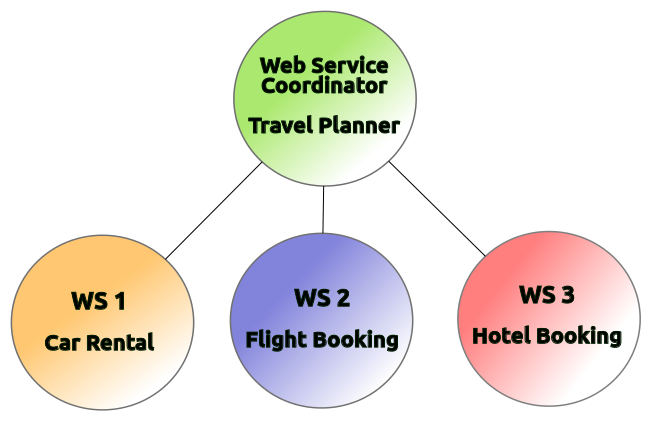
\includegraphics[scale=0.32]{pictures/FigOrchestration}
\label{fig:orchestration}
}
\hspace{2mm}
\subfigure[Service choreography. The services here collaborate to realize the main objective.]{
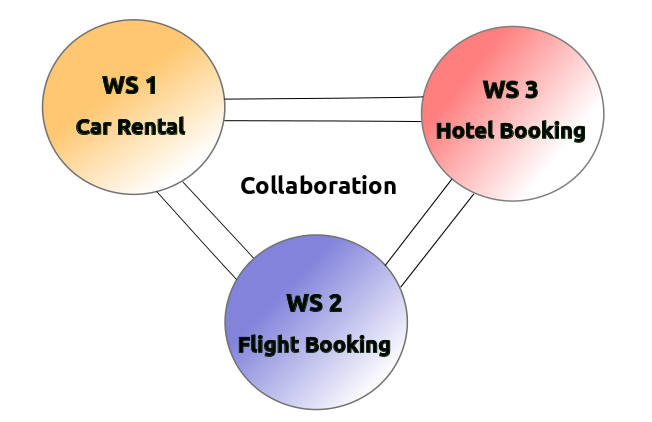
\includegraphics[scale=0.32]{pictures/FigChoreography}
\label{fig:choreography}
}
\caption{Example of service orchestration versus service choreography}
\label{fig:OrchAndChor}
\end{figure} 
%%%%%%%%%%%%%%%%%%%%%%%%%%%%%%%%%%%%%%%%%%%%%%%%%%%%%%%%%%%%%%%

%\subsection{BPEL} FIXME: review!
\subsection{BPEL - The Overview} \label{BPEL}

In today's interconnected world, companies and businesses need to exchange data effectively and get communication flow as fast as possible, in order to save time and be more competitive. They want to automate their business processes and speed up the information exchange. BPEL is a standard that can help them to achieve this goal.
BPEL (which stands for Business Process Execution Language) is an XML standard for describing and defining business processes and hereby standardize the format of information exchange between different softwares. 

BPEL was initially developed by IBM and Microsoft. Its first version (1.0) was released in 2002 by these companies and BEA. Developers wanted to merge IBM's WSFL and Microsoft's XLANG. Both WSFL and XLANG have the same purpose - to combine web services in supporting business processes. During the following year, other companies (Siebel Systems and SAP) joined the development of BPEL and one year later they released version 1.1 together. After this, BPEL was passed to the OASIS nonprofit consortium. In 2007 Web Services BPEL (WS-BPEL) version 2.0 standard was released. During the year 2005 OASIS announced development of extension of WS-BPEL called BPEL4People, including the human interaction in BPEL processes \cite{BPELonWikipedia}.



\paragraph{BPEL Architecture example} \label{BPELarchitecture}
This paragraph contains a brief example of a simple BPEL server and its description. 
In a typical, scenario BPEL process is run on some BPEL engine which is accessible through web services (which among other things contributes to BPEL Architecture platform and operating system independence). After deploying the process, the engine waits for a request (WSDL messages) from clients (which can be for example another BPEL server or a web interface). After the request is received, the BPEL engine creates an instance of a BPEL process and runs it. When running, the process can further interact with the client and also with different BPEL servers. At the end of the operation the result is sent to the client and the process is destroyed in the server.
Note that this is not a general case since BPEL specification does not include any description of the architecture of a BPEL system and therefore this part serves for a reader to get an idea of how BPEL process works (see Figure \ref{BPELprocess}).  

\subsubsection{BPEL Activities} 
\label{BPELActivities}

In a BPEL process, activities are used to define the process logic. Activities are divided into two classes: basic and structured. 

\begin{enumerate}
\item Basic activities are those which describe elementary steps of the process behavior. The following is a list of the most important ones:
	\begin{itemize}
	\item \verb|<invoke>|
	\item \verb|<receive>|
	\item \verb|<reply>|
	\item \verb|<assign>|
	\item \verb|<throw>|
	\end{itemize}

\item Structured activities encode control-flow logic, and can contain other basic and/or structured activities recursively. The most important are listed below:
	\begin{itemize}
	\item \verb|<sequence>|
	\item \verb|<flow>|
	\item \verb|<if>|, \verb|<while>|, \verb|<repeatUntil>|  
	\item \verb|<pick>|
  \end{itemize}
\end{enumerate}


\subsubsection{BPEL Communication}
\label{BPELCommunication}
BPEL processes need to communicate with each other and for this purpose they usually use the combination of a description language, WSDL (see section \ref{Wsdl}), and a protocol, SOAP. WSDL stands for Web Services Description Language and is used to define the interfaces between communicating processes. It means that WSDL determines the format of messages, their data types and types of ports used for transmitting messages \footnote{each port has a particular type(s) assigned and therefore it can receive/send messages of this type(s) only} Whereas WSDL defines the interface between processes, SOAP works on lower level and is used for transmitting the data.

\begin{figure}
\begin{center}
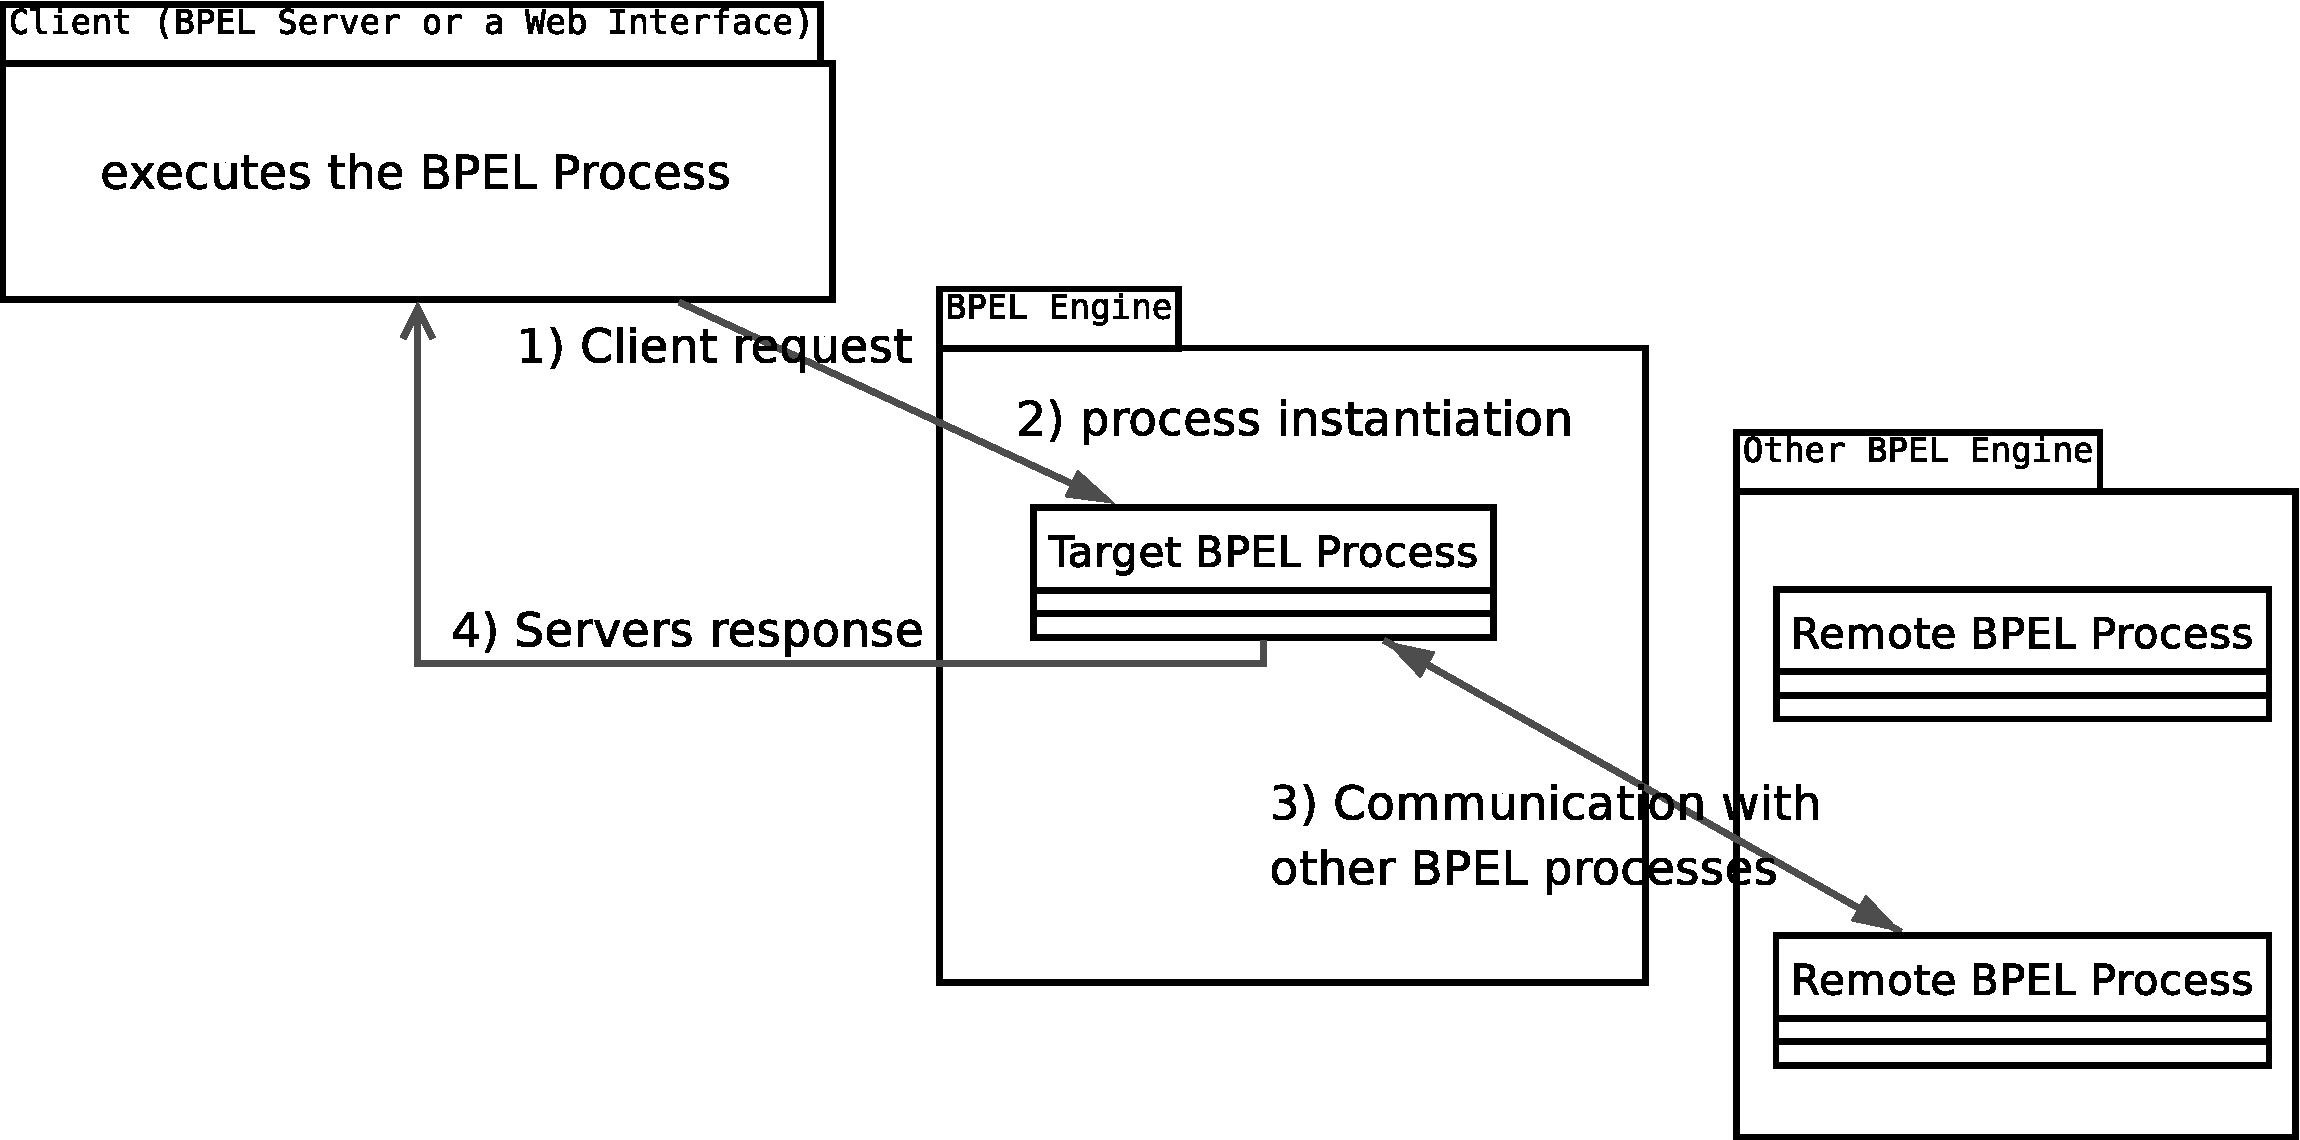
\includegraphics[width=125mm]{pictures/image-BPEL.pdf}
\caption{ Execution of a simple BPEL Process \textbf{FIXME(To Realize with UML Deployment Diagram)}}
\label{BPELprocess}
\end{center}
\end{figure}

\subsubsection{Technologies and protocols used by BPEL}
As mentioned before, BPEL uses WSDL to define process interface and SOAP for message transmitting. On lower levels XML Schema is used for defining the type of XML documents which are sent and received. On the lowest level XML is used for data encapsulation. This can also vary from implementation to implementation. For example, some engines (i.e. Oracle BPEL Process Manager) allow communication with each other using Java RMI instead of SOAP. WS-BPEL 2.0 standard also adds in the specification some new technologies like XPath for accessing data in complex variables and XSLT operations for transforming them \cite{OraBPELRMIInvocation}.


\label{BPELfiles}
BPEL is based on the XML language. As a programming language it has three basic components: the programming logic, the data types and the input/output (I/O). They are divided into three files written in three languages: BPEL, XML Schema definition and WSDL. 
The BPEL file contains the "orchestration" of the system. It specifies an executable process that involves message exchanges between the various processes composing the system. The XML Schema file is used to define the types used in the program. The WSDL file defines the Web Service from an "abstract" point of view describing all the operations for each process participating in the business service.
Table \ref{BPELfilesTable} summarizes the functionalities of the three files composing a BPEL process.

%%%%%%%    Table %%%%%%%%%%%%%%%%%%%%%%%%%%%%%%%%%%%%%%%%%%%%%%
\begin{table}[h!]
\caption{BPEL files' functionalities}
\label{BPELfilesTable}
\begin{center}
\begin{tabular}{l l l}
						\toprule
						\addlinespace[0.2cm]
\textbf{Basic Components} 	& \textbf{Language} 	& \textbf{File extension} 	\\ 
						\cmidrule(l){1-3}
Programming Logic 		& BPEL			& .bpel 			\\[0,1cm]
Data Types 			& XSD (XML Schema) 	& .xsd 				\\[0,1cm]
Input/Output 			& WSDL 			& .wsdl 			\\[0,1cm]
						\addlinespace[0.2cm]
						\bottomrule
\end{tabular}
\end{center}
\end{table}
%%%%%%%%%%%%%%%%%%%%%%%%%%%%%%%%%%%%%%%%%%%%%%%%%%%%%%%%%%%%%%


\paragraph{BPEL Engines}
Table \ref{BPELengines} represents several common BPEL engines developed by various companies \cite{BPELenginesComparisonOnWikipedia}. In this document we do not go deep into the engines' details as we concentrate more on the BPEL process, its orchestration and its functionalities. Of course, sometimes it is not possible to explain BPEL concepts without a basic knowledge about the engines. Thus, brief explanations are provided when necessary.


%%%%%%%%% Table %%%%%%%%%%%%%%%%%%%%%%%%%%%%%%%%%%%%%%%%%%%%%%%%%%%%%%%%%%%
\begin{table}
\caption{List of BPEL engines}
\label{BPELengines}
\begin{center}
\begin{tabular}{l l l}  %\begin{tabular}{|p{5.5cm}|p{3cm}|p{2.5cm}|}
						\toprule
						\addlinespace[0.2cm]
{\bf Name of BPEL Engine} 	& {\bf Supported BPEL Version} 	& {\bf License} 	\\
						\cmidrule(l){1-3}
ActiveBPEL         		& BPEL4WS 1.1, WS-BPEL 2.0 	& GPL and commercial 	\\[0,1cm]
Apache ODE         		& WS-BPEL 2.0 			& Apache license	\\[0,1cm]
jBMP (jBoss)         		& WS-BPEL 2.0 			& LGPL			\\[0,1cm]
Open ESB (Oracle)		& WS-BPEL 2.0 			& Open Source		\\[0,1cm] 
Oracle BPEL Process Manager   	& BPEL4WS 2.0 			& commercial		\\[0,1cm]
WebSphere Process Server (IBM)	& WS-BPEL 2.0			& commercial		\\[0,1cm]
						\addlinespace[0.2cm]
						\bottomrule
\end{tabular}
\end{center}
\end{table}
%%%%%%%%%%%%%%%%%%%%%%%%%%%%%%%%%%%%%%%%%%%%%%%%%%%%%%%%%%%%%%%%%%%%%%%%%%%

%\subsection{Java RMI} FIXME: review!
% Literature review: Summary of Java RMI
% Author: Pierre

\subsection{Java RMI} \label{JavaRMI}   

\textit{Java RMI}, as the name suggests, is an extension of the Java object model, that provides support for distributed objects in the Java language. The remote method calls are done using the same syntax as for local calls, the only difference is that the object making the invocation is aware that its target is remote, as it must handle \textit{RemoteExceptions}. On the other hand, the implementer of a remote object is aware that it is remote because it must implement the \textit{Remote} interface. In order to fill this section we used the Java RMI technology overview \cite{RMI-sun} and the tutorial from the SUN website \cite{RMI-client-sun} and \cite{RMI-overview-sun}.

\paragraph{Remote Interfaces in \textit{Java RMI}}

Remote interfaces are defined by extending an interface called \textit{Remote}, provided in the \textit{java.rmi} package. The remote methods must throw a \textit{RemoteException} in addition to any application specific extension. A remote interface can receive both ordinary and remote objects as arguments, which is also true for its results.

\paragraph{Parameter and result passing}

The arguments of a method are described as \textit{input}, whereas the result is a single \textit{output} parameter. Any object implementing the \textit{serializable} interface (thus being serializable) can be passed as an \textit{input} or \textit{output} in Java RMI.
When the type of a parameter or result value is defined as a remote interface, the corresponding argument or result is always passed as a remote object reference. On the other hand, when a remote object reference is received, it can be used to make RMI calls on the remote object it refers to.
All serializable non-remote objects are copied and passed by value. This way, a new object can be changed locally, possibly causing its state to differ from the one of the original object.

\paragraph{Downloading of classes}

Thanks to Java's virtual machine, classes can easily be transferred from one system to another. This feature is quite useful when placed in the context of distributed objects communicating through remote invocations. If a recipient does not possess the class of an object that has been send to it, the fitting code is downloaded automatically. This allows clients and servers to make transparent use of instances of new classes whenever they are added. Furthermore, there is no need for users to keep the same set of classes in their working environment.

\paragraph{RMI registry}

RMI registry is the middleware in charge of the binding tasks in \textit{Java RMI}. It has to be run on every server hosting remote objects. The RMI registry is actually in charge of maintaining a mapping table associating symbolic object names with remote objects hosted on this computer. It is accessed by methods of the \textit{Naming} class :
\begin{description}
\item[static void 	bind(String name, Remote obj)]
    Binds the specified name to a remote object.
\item[static String[] 	list(String name)]
    Returns an array of the names bound in the registry.
\item[static Remote 	lookup(String name)]
    Returns a reference, a stub, for the remote object associated with the specified name.
\item[static void 	rebind(String name, Remote obj)]
    Rebinds the specified name to a new remote object.
\item[static void 	unbind(String name)]
    Destroys the binding for the specified name that is associated with a remote object.
\end{description}
These methods take a string formatted in the following way as an argument:
\verb|//computerName:port/objectName|
where \textit{computerName} and \textit{port} refer to the location of the RMI registry.
\cite{DS-book}

% New part added by Antonio
% FIXME - I don't know the source of the following text. I need it for citations... I had a look to the "cite" at the beginning of this section, but no source of them fits to it..... :(

\subsubsection{Java RMI Architecture} 
\label{JavaRMIArchitecture}

\paragraph{Interfaces}
\label{JavaRMIinterfaces}
The RMI architecture is based on one important principle: the definition of a behavior and its implementation are separate concepts and their code run on separate JVMs. Moreover, the behavior is described in a Java Interface whereas the implementation is coded in a class \cite{RMI-art5}.
The Java Interface, containing the behavior, runs on the server. There are two implementations of this interface:
\begin{itemize}
	\item On the Server: Behavior's implementation class
	\item On the Client: Proxy class object
\end{itemize}

The client makes method calls directly on the proxy class object, then the proxy sends the request to the server's JVM which contacts the implementation. Any return values are sent back the other way around.

\paragraph{RMI architecture layers}
\label{RMIarchitectureLayers}

\begin{figure}
\begin{center}
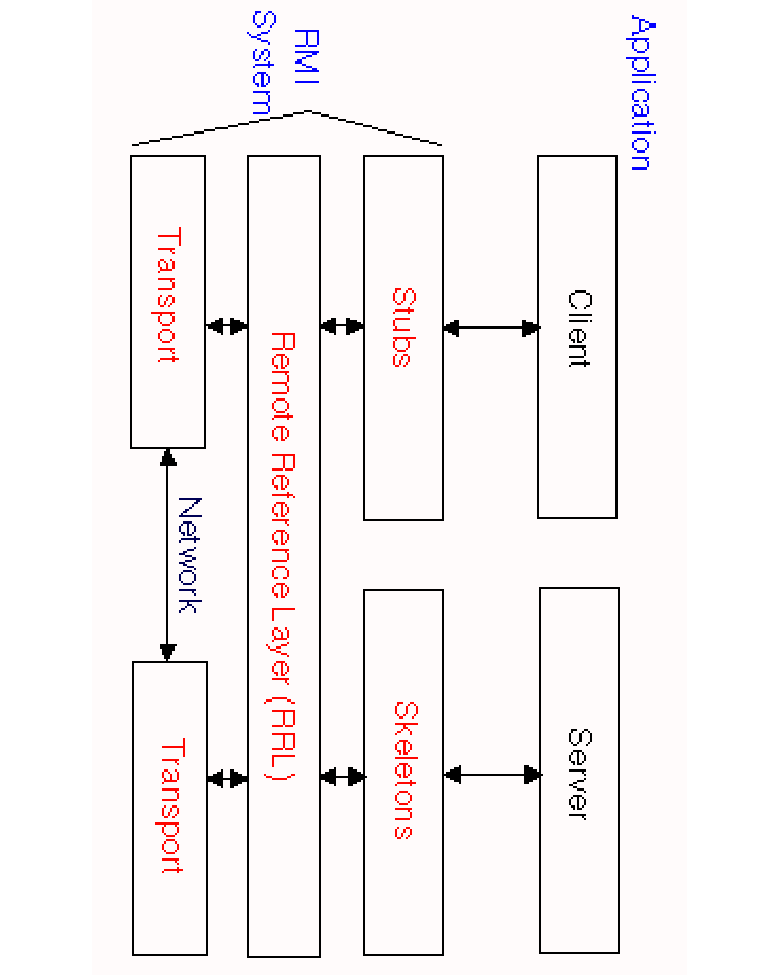
\includegraphics[angle=90, scale=0.65]{pictures/rmi.pdf}
\caption{The layers of RMI}
\label{RMIlayers}
\end{center}
\end{figure}

The RMI implementation is built by three abstract layers shown on Figure \ref{RMIlayers}:

\begin{enumerate}
\item Stub/Skeleton
\item Remote Object Reference
\item Transport Layer
\end{enumerate}

\subparagraph{The Stub and Skeleton layer}
From the client's point of view the Stub object is a proxy which receives all requests directed to the server's service. The Skeleton, on the server side, does almost the same: receives the request from the Stub and passes it to the "real" object containing the method's implementation. Stub and Skeleton don't make any calculation or change on parameters, they just contain the code to communicate to each other. This avoids having to write the implementation of the "communication channel" directly in the client or server Java file. This is why the method's calls look like so similar to local calls. From the JDK 1.2 the Skeleton is not used anymore.
\subparagraph{The Remote Object Reference layer}
The Remote Object Reference layer provides a \verb|RemoteRef| object that represents the link, for the stub, to the class containing the implementation on the server. 
\subparagraph{The transport layer}
The transport layer makes the connection between JVMs and it uses the TCP/IP protocol. Even if two JVMs, containing two different services, are running on the same physical machine, they will connect through the TCP/IP protocol stack. 

%**********************************************************************************

\subsubsection{Java RMI: The Internal Mechanism}
\label{JavaRMIinternalMechanism}

This section concretely explains how Java RMI works and how it can 
help programmers in the writing of the network related code in their programs.

A typical scenario could be: a client wants to execute a method on the server which is on another machine. We will explain why the programmer does not have to write the network and sockets code with Java RMI.

We know that for the service interface on the server, there are two implementations with the same methods: the Stub on the client side and the real object implementing the behavior on the server side. In particular the client uses the stub to call all the methods the same way it would call them on the server. The only difference with a local call is that the stub does not contain the concrete implementation of the required function, it just contains the network-related code to create the communication channel with the server's real implementation \cite{RMI-art4}.
%Thus, from the JDK 1.2, there will be three classes: the client, the stub and the server's real implementation.     
%Client<--->stub<--->[NETWORK]<--->Server_real_implementation.

\paragraph{Socket-Level Details}
\label{SocketLevelDetails}

The following is the list of steps executed by a Java RMI program for each method's call:
\begin{enumerate}
\item The server object listens on an anonymous port on the server machine. The port is chosen at runtime by the JVM or the OS.
\item The client does not know the particular port on the server where the object is listening. It calls the method locally on the stub.
\item The stub creates a TCP/IP communication channel between client and server and it works in 5 steps: 
	\begin{itemize}
	\item The client connects to the server's listening port (see the Bootstrap problem paragraph to understand how the          Stub can know the server's address and port).
  \item The server, waiting for a client's request, accepts the incoming connection and creates a new socket just to 				  handle this single connection.
  \item The server will continue to use the old listening port to wait for other incoming requests.
  \item The communication between client and server takes place using the newly created socket on the server.
  \item They communicate and exchange parameters and results with an agreed-upon protocol. The protocol can be                 \textit{JRMP} (Java Remote Method Protocol) or CORBA-compatible \textit{RMI-IIOP} (Internet Inter-ORB                  Protocol).
	\end{itemize}
\item The method is executed on the server's real implemented object and the result is sent back to the stub.
\item The Stub returns the result back to the client object as if the stub had executed the method locally.
\end{enumerate}

\paragraph{Bootstrap problem}
\label{BootstrapProblem}
In point 2 of paragraph \ref{SocketLevelDetails} we did not explain how the stub on the client side can know the anonymous port where the object is listening on the server. The client has to know at least the IP address of the server machine where the service is available; thus the only problem for the client side is to get the anonymous port.
The RMI registry is used for this purpose: it stays on the server and keeps the correspondences between the name of the service and its address, in a table.
The Registry keeps pairs of $<$public\_name, Stub\_object$>$ in a hashmap, where:
\begin{description}
\item [public\_name] is the name attributed by the server to the implemented object.
\item [Stub\_object] is an instance of the Stub object containing also the address of the anonymous port. 
\end{description}

The following list explains how the Bootstrap problem is solved in Java RMI:
\begin{enumerate}
\item The RMI registry is also a Remote Object and listens on a well-known port on the server machine, by default the 1099.
\item The server creates an object (we call it the \textit{ServiceObject}) listening on an anonymous port.
\item The server automatically creates a \textit{Stub\_ServiceObject} of the new \textit{ServiceObject}
\item When \textit{rebind(String name, Remote obj)} is called on the server side, it passes a Remote Object Reference of the \textit{ServiceObject}, containing the exact port address, as the second parameter. The RMI registry Naming class constructs a new stub object in the registry by copying the already existing \textit{Stub\_ServiceObject} on the server machine and by adding the Remote Object Reference to it.
\item Now there is a pair $<$public\_name, Stub\_object$>$ in the RMI registry containing the name of the service and a Stub object also containing the "real" address of the \textit{ServiceObject} on the server.
\item When the client executes Naming.lookup(public\_name) (e.g \\ Naming.lookup("rmi://Server\_IP\_address:1099/calc") ) it passes the public name as the parameter to the RMI registry on the server. 
\item The RMI registry returns the stored \textit{Stub\_object} object back to the client. Now, the client gets a stub object that knows about the server's host name and port to which the server listens.
\item Now the client can just invoke the \textit{Stub\_object}'s method which will call the same method of the \textit{ServiceObject} on the server.
\end{enumerate}

After all these steps the client and the server don't need the RMI registry anymore. Actually, instead of the Registry, programmers could use different solutions to let the client know about the server's port where the \textit{ServiceObject} is listening, but we will not go into the details of these techniques. 
About the stub, we could say that it is the core of the RMI mechanism. After the Bootstrap it permits programmers to get rid of the communication protocol between client and server and to easily make remote calls like local calls.

%- Overview, features. - Why? it can run everywhere, lightweight scenarios.
%\subsection{Jet}
%\subsection{EMF and Open Architecture Ware (Eclipse)}
%\subsection{other...} 


% %---Where the problem is---
% \subsection{BPEL, its drawbacks and the use of WSs in a lightweight scenario}
% %\subsection{The drawbacks of using BPEL (BPEL and its possible drawbacks)}
% - BPEL, the de-facto standard concerning web services composition. \nl
% - Overview and brief review\nl
% - What do we use of it, the whole language or just a part? \nl %Questo dove andrà??
% - Problems: It works over Distributed Systems, engine powerful but heavy, DS not always available. \nl %i problemi che ha in generale e quelli specifici al nostro caso
% 
% %---Why we face the problem and which is the possible solution (and aim of the work)---
% %\subsection{Web Services Composition in lightweight scenario}
% - That's our question \nl
% - Sometimes we might need services composition working in less powerful environments than distributed systems. Examples? \nl
% - But we don't want to create a new application from scratch neither...(change hardware?).  \nl




%---Introduction to the MDA and how it basically works
\section{Model Driven Engineering (MDE)}
\label{ModelDrivenEngineering}
Model Driven Engineering (MDE) is a development methodology which focuses on creating models rather than algorithmic concepts that are usually addressed in the classical programming approaches.
This discipline attempts an abstraction of the benefits and the features provided by the Software Engineering \cite{Marrone}, usually creating a domain specific framework for implementing new systems, based on well known and tested concepts, obtained through a careful and detailed analysis of the domain and its actors.\\
%
MDE essentially shifts the focus from the program code to models, making them the gravitational center of every MDE process \cite{Lukman08}. The model represents the system and the language which describes the model must be characterized by a well defined syntax and semantic. This way, if the model strictly complies with the languages' rules, it is possible to create automatized routines that carry out activities such as debugging, validation, simulation or transformation \cite{Papa11}. 
The language to describe the model is itself complying with a meta-model which, recursively, complies with a meta-meta-model. In fact, a typical MDE approach consists of the usage of a pile of models having at the top the system model. \\
%
Eventually, the two main principles of MDE are:
\begin{itemize}
 \item creation of models: using meta-modelling techniques
 \item automatized manipulation of models: using transformations to transform an input model (conforming to a source meta-model) to an output model (conforming to a destination meta-model)
\end{itemize}

\subsection{Model Driven Architecture (MDA)}
\label{MDA}
Actually, the MDE concepts are generic and can be applied to many engineering disciplines where models are used. To narrow our attention down to software development, we should consider the Model Driven Architecture (MDA), which is a standard from the Object Management Group (OMG) that specifies in details the particular modeling languages (e.g. UML) and the related automations to map an input model into an output one.
A very common MDA pattern consists of the definition of three models \cite{Marrone} representing the input application, the platform information and the output application:

\begin{itemize}
 \item Platform Independent Model (PIM): it is a model of the application, completely independent from the platform on which it might be implemented
 \item Platform Description Model (PDM): it describes the architecture on which the output application should be deployed
 \item Platform Specific Model (PSM)$=f($PIM,PDM$)$: it is the result of an automatic transformation of the PIM using the PDM specific platform directives  
\end{itemize}

The output models, result of the MDA transformations, are so called: "correct-by-construction" models, in opposition to some traditional transformations that are of a "construct-by-correction" type \cite{Marrone}.   


\subsection{MDA: the manipulation of models}
\label{MDAModelManipulation}
Among the automated routines that MDA can perform on models, we focus on the model Transformations, that, starting from an input model, create an output model conforming to a destination meta-model. 

\paragraph{Transformations of models}
As described in \cite{Papa11}, a transformation is formed by a set of rules, or \textbf{transformation rules}, that describe how an element expressed in the source language should be transformed in one or more elements of the destination language.
Of course, both the source and destination model must comply with their respective meta-models.
%FIXME add a picture like the one in http://www.ebpml.org/blog/130.htm
The possible transformation rules that can be applied to a model depend on the approaches being used \footnote{Some approaches come from the scientific literature, some in response to the OMG's requests for proposals and others from open-source or commercial vendors.}. Czarnecki and Helsen \cite{Czarnecki03classificationof} classify and describe the set of rules common to all the approaches.
They individuate the main rules that compose a model transformation. The rules span from the ones defining how to transform and with which scope to the ones about scheduling and organization of the transformation.

\subsubsection{Model-to-Model and Model-to-Text transformations}
\label{m2m&m2t}
Depending on the kind of source model\footnote{other techniques, not model-based (XML document to XML document, Text-to-Binaries, etc.), can also be abstracted under the generic type of model transformations \cite{M2TandM2M}} , there are two kinds of transformations \cite{Papa11}: \textbf{Model-to-Model} and \textbf{Model-to-Text} (or Model-to-Code, when the output text is a programming language syntax.). Both the transformations can be implemented in two ways \cite{M2TandM2M}:
\begin{itemize}
 \item Using a model Domain-Specific Modeling Language (DSML)
 \item Using a General Purpose Language (GPL), e.g. Java, C\#
\end{itemize}
The difference is that a domain specific modeling language focus on a particular application domain thus it can represent concepts that are not possible to describe with a general purpose language.

\paragraph{Model-to-Text approaches}
If we have a deper look in the Model-to-Text transformations, we notice that Czarnecki and Helsen \cite{Czarnecki03classificationof} subdivide this category in two: Visitor-based and Template-based transformations.
\subparagraph{Visitor-Based model-to-text transformation}
It is a simple method where a visitor mechanism can traverse the model's internal architecture and directly write text as output, deciding what transformation to apply depending on the construct encountered. 
\subparagraph{Template-Based model-to-text transformation}
This approach represents the most used M2T technique. It contains code templates in which some portions of code are left blank, waiting to be filled with information coming from the input model. 
The templates comply to the output meta-model, and resembles the code to be generated. 
In the template-based transformations, there also are multiple mechanisms to gather the information (from the source model) to insert in the templates. A common way is to describe the source model with a non-ambiguous language and later access it through an API provided by the creators of the modeling language. Declarative queries can also be used, as it happens with the Object Constraint Language (OCL) or XML PAth Language (XPath). 
More advanced techniques implement a hybrid solution, using a mix templates and more complex queries to get data from different parts of the source model.  
\fxnote[inline=true]{I templates in Acceleo sono scritti nel linguaggio di destinazione (Java nel nostro caso) + snippets di codice Acceleo. In generale, i templates sono (sempre?) scritti nel linguaggio di destinazione? 


% Acceleo M2T
\subsection{Acceleo FIXME: to move and complete}
\label{acceleo}

General Info about meta-modelling   :Pag7 \cite{AcceleoUserGuide}

- MEtamodelling is a vast domain
--- MetaModelling has been formalizaed by OMG, known as MOF Meta-Modeling Facilities
----- MOF is itself a model, represented as a tree. It is considered a meta-meta-model as it can be used to describe many other meta-models. This is possible thanks to the fact that its components are basic, and form the atomic pieces used to create other models. 
For example, if a map represents a model of a region, existing in the real world, its meta-model would contain the basic elements to represent such a map, namely, a legend. This meta-model would contain elements such as roads, highways, rivers, cities, villages etc. In this context, a meta-meta-model would go further deep in the description, containing the structure of the atomic elements to represent the elements of the meta-model (the legend). For example, of a river, it would present a modelization of it, containing name, depth, length and more.  

Basically, a model is an instance of a meta-model \cite{UnderstandMetamodelling}. 


---- XMI is the standard from OMG to transform, interchange, and express any model realized with the MOF.   
   

% The best known MDE initiative is the Object Management Group (OMG) initiative Model-Driven Architecture (MDA), which is a registered trademark of OMG \cite{MDE}.
% 
% It is generic and groups all of the more specific techniques to develop something using models. This something can be software, ...etc.
% The objective: define methodologies and techniques to support software development through models manipulation.


% \subsection{The Model Driven Architecture (MDA)}
% \label{MDA}
% 
% \subsubsection{Model Driven Engineering}
% \label{MDE}
% \subsubsection{Model to Text transformation (M2T)}
% \label{M2T}
% \subsubsection{Acceleo}
% \label{Accelelo}

%- What it is \nl
%- Why we use it, why is good (because it is generic, Architecture independent, Reuse)  \nl
%- How we use it: From BPEL processes to Java RMI processes \nl

 

% How we do it: Why we do it, What particular method we use and what logic architecture we use
\section{The methodological approach}
\label{MethodApproach}
%---What methodology we used---

We analyze the possibility of automatically transform a BPEL written process in a Java executable routine, with minimum ad-hoc developer’s intervention. Our final objective is to show the feasibility of a semi-automated transformation from a small business process orchestrated with BPEL to the Java language.
This section describes the methodological approach we undertaken to realize our objective. The following list summarizes the steps we undertake to make our final choice:

\begin{itemize}
 \item The domain of our transformation
 \item  The methodological approach: Programming vs Code Generation vs Model Driven Architecture 
 \item Choose a model driven architecture that allows us to manipulate  the BPEL input model (M2M, M2T) and that is compatible with a ready to run code output.
 \item We identify the subset of BPEL instructions suitable for a proof of concept of the transformation.
 \item Select a BPEL meta-model that covers the chosen subset of instructions.
 \item Individuate a BPEL workflow pattern to work on 
\end{itemize} 

Once these steps have been accomplished, we focus on providing more details on how we carry out the transformation. The main points are:
\textbf{DA SCRIVERE NELLA SEZIONE DETAILED ARCHITECTURE ? }
\begin{itemize}
 \item Provide a correspondence from BPEL constructs to Java concepts
 \item Design the structure of the output application.
 \item Define the essential skeleton of Java classes necessary to create a runnable BPEL process
 \item In the templates, describe how to use and where the dynamic information taken from the BPEL input model has to be placed.
 \item Plan where and how, in the architecture, the developer intervention has to take place.
 \item \textbf{Issues encountered and proposed solutions  ? }
\end{itemize} 
 
 To mention later: \\
 StubPartnerLinks, code to be input by the user, static code, the problem with the WSDL file

\subsection{The domain of the transformation} 
In our transformation we are dealing with BPEL, which is a DSL (Domain Specific Language), and Java, which is a multipurpose language. 
Having to deal with a model produced with a DSL means that   we don't have to take care of the general constructs and ideas that are present in a generic language. The language is already skimmed to what is necessary to orchestrate business processes, nothing more.  %Most importantly, the fact the input model is produced in a DSL  
 
\subsection{The methodological approach}
\label{sec:ProgrammingVsMDE}
To realize the transformation, many possibilities arise; from a very specific, custom solution to a more broad and abstract approach. The possibilities could be generalized in three main families: a manual ad-hoc programming solution, a code generation automation or a model driven architecture abstraction
\subsubsection{Ad-hoc Programming solution}
The programming solution would create an ad-hoc solution for our purpose.  At the same time, as our purpose is to provide a proof of concept for our approach more than a runnable application, programming a one time, ready to deploy solution, does not fid our needs.
\subsubsection{Code Generation}
This solution is aimed at automatizing the generation of code that would otherwise have to be written by hand. It concerns the creation of models/templates that will be later transformed in working code by an additional application. Although this solution might partially fit our need of an automated generation, we might have to create models/templates for many components, and we have to take into account a possible large amount of similar portions of code needed in different parts of the final application.  Thus, we need a solution that will rise of one more step the abstraction.
\subsubsection{Model Driven Architecture (MDA) Abstraction}
The MDA aims, as well as the Code Generation automation, at the creation of models to be later transformed in runnable code (see Section \ref{MDA}). The difference lies in the fact that MDA permits to create an architecture where we could actually specify generic transformations strategies. For example, instead of creating a template for any BPEL construct, with MDA we could create a hierarchy of templates where similar BPEL constructs are sharing part of the code minimizing the quantity of hand written code at the price of a longer design phase.
\subsubsection{The proposed methodological approach}
Given the fact that our transformation has the purpose of showing the feasibility of such a transformation form BPEL to Java, we have to take into account that only a small part of the BPEL language can be taken into account. Moreover, we want to propose a possibly expandable design for such a transformation. Last but not least, we have to keep an eye on possible future developments. For these reasons, we decided to use a Model Driven Architecture methodology.

\subsection{Tailoring the MDA approach to our case}
Once the MDA approach has been chosen, we have to choose which kind of model transformation we want to apply.

\subsection{The BPEL subset of instructions}
\label{Sec:BPELsubset}
The BPEL standard (see Section \ref{BPEL} for more details) has a wide variety of elements and instructions aimed at managing the possible workflow patterns obtainable during a services orchestration. Moreover, BPEL does not restrict the number of services that can participate to the orchestration neither the type and the quantity of interactions among them.
For these reason, we focus our attention on a subset of the whole BPEL language, both to restrain the complexity and to fit the time frame of the project.
\subsubsection{The activities subset}
We decided to restrict the BPEL activities to a subset containing the following constructs divided in four groups:
\begin{center}
\begin{supertabular}{p{0.4\textwidth}p{0.4\textwidth}}

1. Basic activities: 			& 2. Structured activities:		\\
\begin{itemize}
	\item \verb|<invoke>|
	\item \verb|<receive>|
	\item \verb|<reply>|
	\item \verb|<assign>|
	\end{itemize} 			&

					    \begin{itemize}
					      \item \verb|<sequence>|
					     \end{itemize}			\\
					     
3. Elementary operations: 		& 4. Static descriptive elements:	\\					
\begin{itemize}
	\item \verb|<copy>|
	\item \verb|<from>|
	\item \verb|<to>|
  \end{itemize} &

					    \begin{itemize}
					      \item \verb|<process>|
					      \item \verb|<partnerLink>|
					      \item \verb|<variable>|
					      \item \verb|<expression>|
					    \end{itemize}\\
\end{supertabular}
\end{center}

The Basic and Structured activities define the BPEL process logic (see Section \ref{BPELActivities}). The elementary operations are present inside the activities, while the static descriptive elements are meant to statically describe some of the parameters needed by BPEL process.
These elements allow the creation of simple BPEL processes, where the activities such as: invoking a service or waiting for a reply, happen as a sequence, one after the other. Although this limits the expressive potentiality of BPEL, it fits our need of focusing on proving the feasibility of an automated transformation from BPEL to Java without having to deal with the complexity of the whole language.
In Figure \ref{fig:SubSetBPEL} the BPEL subset of elements used for this project is depicted.

\begin{figure}
  \begin{center}
    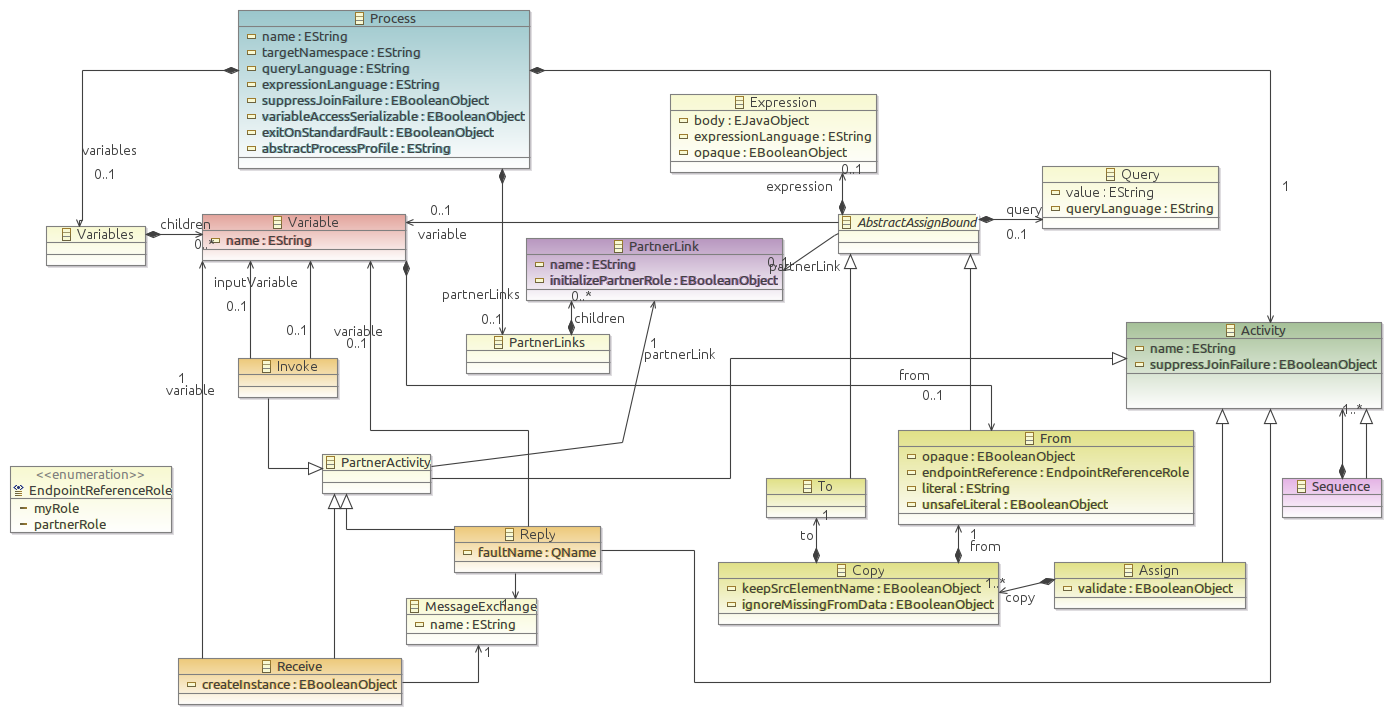
\includegraphics[scale=0.67,angle=90]{pictures/SubSetBpel2.png}
    \caption{The BPEL subset in its ecore model representation}
    \label{fig:SubSetBPEL}
  \end{center}
\end{figure} 

\subsubsection{The meta-model for the BPEL subset}
\label{Sec:DesignBpelSubset}
To permit the parameterization of the BPEL process input model, we need a meta-model describing our subset. The Eclipse Modeling Framework (see Section \ref{EMF}) provides a meta-model written in ecore for the whole BPEL language; we use only the subset elements of this ecore meta-model.
\subsubsection{The BPEL workflow pattern to focus on}
\label{sec:DesignBPELPattern}
The BPEL language with its wide range of activities and operation, gives the possibility to orchestrate many kind of workflow patterns among the participant services. We concentrate our attention on a process having the following participants:
\begin{itemize}
 \item one partner link representing a client
 \item one partner link describing a web-service
\end{itemize}
and on a simple workflow pattern that concerns the activities shown in Figure: \ref{fig:BPELWorkflowPattern}\footnote{This Figure has been realized using the BPEL designer facilities of Eclipse. Yet not a standard, as the Oasis consortium has not released a graphical standard, many vendors provide very similar graphical notations}. The pattern shown in the Figure includes the following steps:
\begin{enumerate}
 \item the process waits for a client to connect and provide an input
\item reception of the input and its assignation to a variable to forward to the web-service.
\item web-service invocation
\item reception of the web-service's reply and assignation to a variable to be forwarded back to the client
\item final response sent back to the client
\end{enumerate}


\begin{figure}
  \begin{center}
    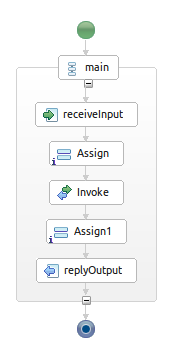
\includegraphics[scale=0.8]{pictures/BPELSimpleProcess.png}
    \caption{The BPEL workflow pattern we focus on}
    \label{fig:BPELWorkflowPattern}
  \end{center}
\end{figure} 
% %\lipsum[2]
% \hvFloat[
%  floatPos=!htb,
%  capWidth=h,
%  capPos=r,
%  capAngle=90,
%  objectAngle=90,
%  capVPos=c,
%  objectPos=c]{figure}{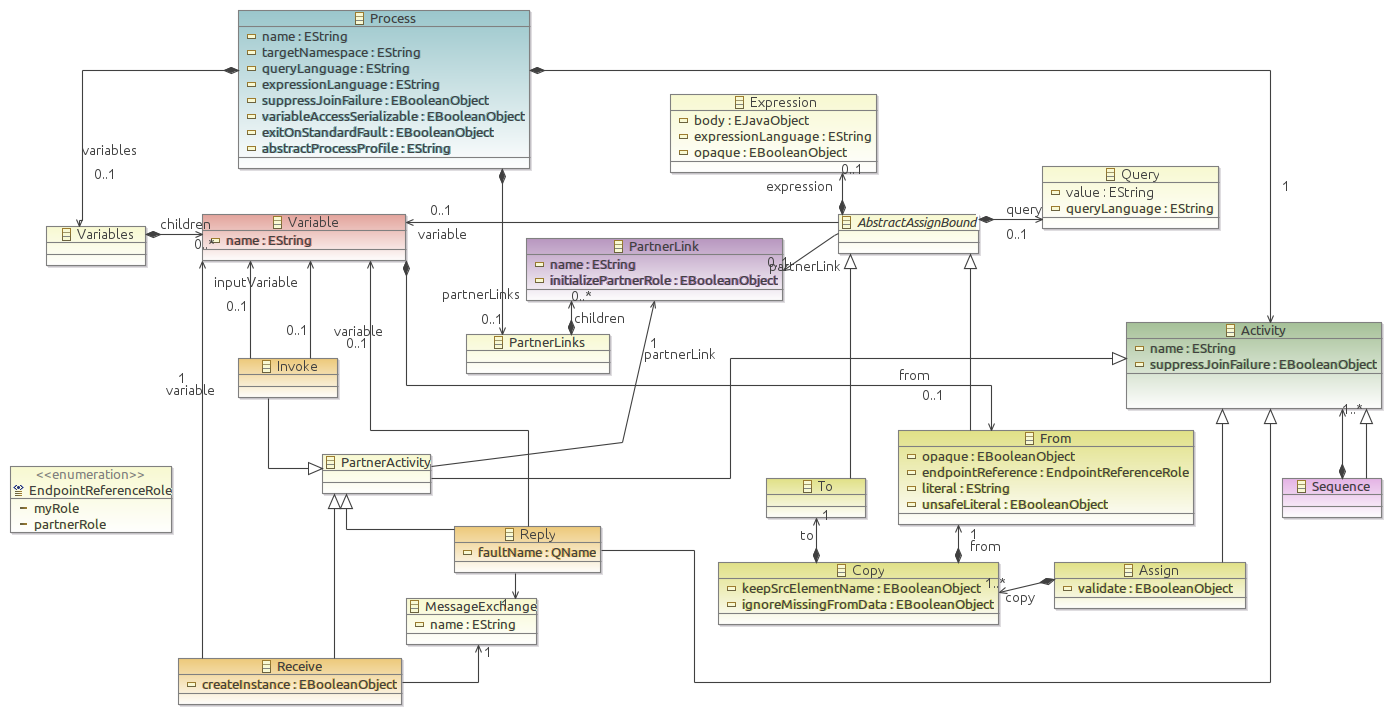
\includegraphics[scale=0.7]{pictures/SubSetBpel2.png}}%
% {Caption vertically centered right beside the float with a caption
% width of figure width and 
% \texttt{floatcapsep=5pt} (the default)}{fig:label}


\begin{figure}
  \begin{center}
    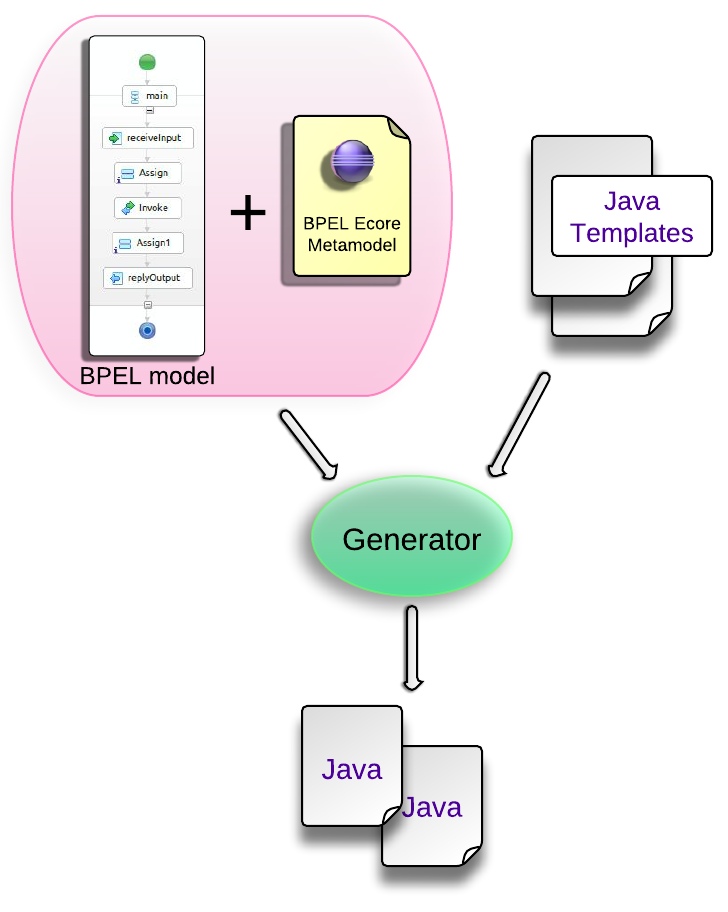
\includegraphics[scale=0.9]{pictures/TransformationApproach.png}
    \caption{The methodological transformation approach}
    \label{fig:TransformationApproach}
  \end{center}
\end{figure}

%----------------------------------------------------


% \begin{multicols}{2}
% \begin{enumerate}
%     \item Basic activities:
%     \begin{itemize}
% 	\item \verb|<invoke>|
% 	\item \verb|<receive>|
% 	\item \verb|<reply>|
% 	\item \verb|<assign>|
% 	\end{itemize}
%     \item Structured activities: 
%     \begin{itemize}
% 	\item \verb|<sequence>|
%     \end{itemize}
%     \item  Elementary operations:
%     \begin{itemize}
% 	\item \verb|<copy>|
% 	\item \verb|<from>|
% 	\item \verb|<to>|
%     \end{itemize}
%     \item Static descriptive elements:
%     \begin{itemize}
% 	\item \verb|<process>|
% 	\item \verb|<partnerLink>|
% 	\item \verb|<variable>|
% 	\item \verb|<expression>|
%     \end{itemize}
% \end{enumerate}
% \end{multicols}
\section{Detailed Architecture}
\label{DetailedArchitecture}
In this Section we introduce the tool we use to realize the chosen methodological approach. In addition, we describe the constraints under which we carry out the transformation, such as the use of a BPEL subset and the specification of a workflow pattern.
Later in this Section, we introduce the design ideas of our transformation and the general architecture we adopted.\\

FIXME: TO REMOVE LATER
\begin{itemize}
 \item *The M2T tool we use (Acceleo)
 %\item The additional components (A WebService)
\end{itemize}

The main points and some more decision we have to take over:
\begin{itemize}
  \item * We identify the subset of BPEL instructions suitable for a proof of concept of the transformation. 
  \subitem * Select a BPEL meta-model that covers the chosen subset of instructions.
  \subitem * Individuate a BPEL workflow pattern to work on 
 
 \item Provide a transformation strategy from the BPEL constructs to Java concepts
 \item Design the structure of the output application.
 \item Define the essential skeleton of Java classes necessary to create a runnable BPEL process
 \item the usage of the wsdl-to-java routine to create the tree of messages types
 \item In the templates, describe how to use and where the dynamic information taken from the BPEL input model has to be placed.
 \item Plan where and how, in the architecture, the developer intervention has to take place.
 \item \textbf{Issues encountered and proposed solutions  ?}
\end{itemize} 
 
 To mention later: \\
 StubPartnerLinks, code to be input by the user, static code, the problem with the WSDL file

\begin{itemize}
 \item Metamodel 
 \item Skeleton 
 \item Generator 
\end{itemize}

%//////////////////////////////////////////////////////////
\subsection{The M2T Generator}
To implement our model-to-text methodology we make use of the Acceleo generator. As described in Section \ref{acceleo}, Acceleo takes as input a model in any kind of modeling language followed by its meta-model descriptor, and a series of templates defining the structure of the output text to create.
With a well defined Acceleo transformations, we can obtain runnable 
Acceleo provides us the opportunity to both navigate the parameterized input model and to plan the design of the Java templates in order not to have redundant code.
%//////////////////////////////////////////////////////////
\subsection{The BPEL subset of instructions}
\label{Sec:BPELsubset}
The BPEL standard (see Section \ref{BPEL} for more details) has a wide variety of elements and instructions aimed at managing the possible workflow patterns obtainable during a services orchestration. Moreover, BPEL does not restrict the number of services that can participate to the orchestration neither the type and the quantity of interactions among them.
For these reason, we focus our attention on a subset of the whole BPEL language, both to restrain the complexity and to fit the time frame of the project.
\subsubsection{The activities subset}
We decided to restrict the BPEL activities to a subset containing the following constructs divided in four groups:
\begin{center}
\begin{supertabular}{p{0.4\textwidth}p{0.4\textwidth}}

1. Basic activities: 			& 2. Structured activities:		\\
\begin{itemize}
	\item \verb|<invoke>|
	\item \verb|<receive>|
	\item \verb|<reply>|
	\item \verb|<assign>|
	\end{itemize} 			&

					    \begin{itemize}
					      \item \verb|<sequence>|
					     \end{itemize}			\\
					     
3. Elementary operations: 		& 4. Static descriptive elements:	\\					
\begin{itemize}
	\item \verb|<copy>|
	\item \verb|<from>|
	\item \verb|<to>|
  \end{itemize} &

					    \begin{itemize}
					      \item \verb|<process>|
					      \item \verb|<partnerLink>|
					      \item \verb|<variable>|
					      \item \verb|<expression>|
					    \end{itemize}\\
\end{supertabular}
\end{center}

The Basic and Structured activities define the BPEL process logic (see Section \ref{BPELActivities}). The elementary operations are present inside the activities, while the static descriptive elements are meant to statically describe some of the parameters needed by BPEL process.
These elements allow the creation of simple BPEL processes, where the activities such as: invoking a service or waiting for a reply, happen as a sequence, one after the other. Although this limits the expressive potentiality of BPEL, it fits our need of focusing on proving the feasibility of an automated transformation from BPEL to Java without having to deal with the complexity of the whole language.
In Figure \ref{fig:SubSetBPEL} the BPEL subset of elements used for this project is depicted.

\begin{figure}
  \begin{center}
    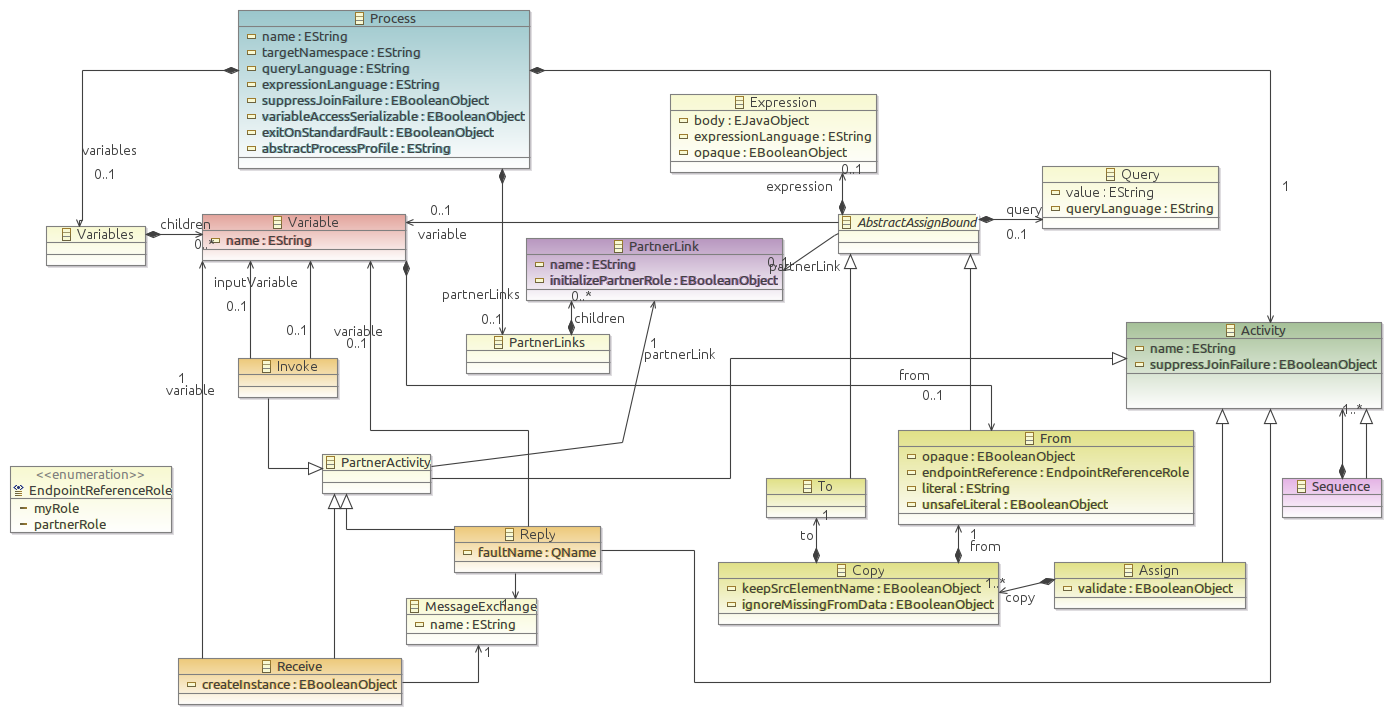
\includegraphics[scale=0.67,angle=90]{pictures/SubSetBpel2.png}
    \caption{The BPEL subset in its ecore model representation}
    \label{fig:SubSetBPEL}
  \end{center}
\end{figure} 

\subsubsection{The meta-model for the BPEL subset}
\label{Sec:DesignBpelSubset}
To permit the parameterization of the BPEL process input model, we need a meta-model describing our subset. The Eclipse Modeling Framework (see Section \ref{EMF}) provides a meta-model written in ecore for the whole BPEL language; we use only the subset elements of this ecore meta-model.
\subsubsection{The BPEL workflow pattern to focus on}
\label{sec:DesignBPELPattern}
The BPEL language with its wide range of activities and operation, gives the possibility to orchestrate many kind of workflow patterns among the participant services. We concentrate our attention on a process having the following participants:
\begin{itemize}
 \item one partner link representing a client
 \item one partner link describing a web-service
\end{itemize}
and on a simple workflow pattern that concerns the activities shown in Figure: \ref{fig:BPELWorkflowPattern}\footnote{This Figure has been realized using the BPEL designer facilities of Eclipse. Yet not a standard, as the Oasis consortium has not released a graphical standard, many vendors provide very similar graphical notations}. The pattern shown in the Figure includes the following steps:
\begin{enumerate}
 \item the process waits for a client to connect and provide an input
\item reception of the input and its assignation to a variable to forward to the web-service.
\item web-service invocation
\item reception of the web-service's reply and assignation to a variable to be forwarded back to the client
\item final response sent back to the client
\end{enumerate}


\begin{figure}
  \begin{center}
    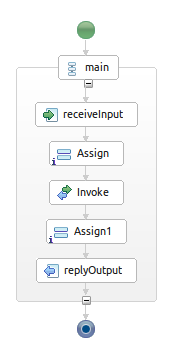
\includegraphics[scale=0.8]{pictures/BPELSimpleProcess.png}
    \caption{The BPEL workflow pattern we focus on}
    \label{fig:BPELWorkflowPattern}
  \end{center}
\end{figure} 

%///////////////////////////////////////////////////////////////
\subsection{Transformation Strategy}
\label{sec:TransformationStrategy}
As a direct transformation from BPEL constructs in Java concepts is neither feasible nor advisable, we have to provide a general strategy tackling single or groups of BPEL activities and creating Java counterparts. The following sections describe the single components of this strategy.

\subsubsection{The input files we work on}
\label{sec:inputFiles}
In a simple BPEL process there are two kind of files containing data valuable for our transformation: the BPEL process description files and the WSDL files to describe the services the process is orchestrating.
The BPEL process files contain: 
\begin{itemize}
 \item the definition of the partner links
 \item the variables used by the process to store or forward information
 \item the orchestration logic.
\end{itemize}
The WSDL files contain, in each file: 
\begin{itemize}
 \item the definition of a service
 \item the basic types used by the service's operations (\verb|<portType>|)
 \item the messages that contain elements of the basic types
 \item the service's definition including its name, server IP and port address. 
 \item the binding definition, which tells how a client could access the service (e.g. using the SOAP protocol)
\end{itemize}

\subsubsection{Translating the WSDL messages structure}
\label{sec:WSDLMEssagesStructure}
A very important feature of our transformation is to be able to generate a data definition specular to the one contained in the WSDL messages definition. WSDL messages can contain, for example, many elements of other types, and these types are, recursively, defined in the WSDL file (Think of a class "office" which contains elements such as "Person", which is a basic type formed by two Strings: "name" and "surname"). 
Instead of taking over the whole task of recreating the messages in Java, we reuse one of the already existing routines to generate the messages structure contained in a WSDL file in Java classes. From the many available, we picked the \textit{wsimport} routine \cite{wsimport}, freely available from the Oracle website. Of the wsimport features, we are interested in the one that translates the xml-written messages types described in the WSDL file in ready to use (and documented) Java classes. The classes and the attributes keep the names used in the WSDL file, making them aligned with the names found in the BPEL process description.
This tool proved very useful as we could make use of a reliable and tested solution, and at the same time concentrate the extra time gained on the transformation's logic. 

\subsubsection{Mimic the BPEL logic}
\label{mimicBPELLogic}
The BPEL orchestration logic is contained in a well defined section of a BPEL file. In the case of our BPEL subset, the logic workflow is all included in the \textit{sequence} activity.
When generating the Java code, we make sure that the instructions included in the \textit{sequence} all end up in a Java class called after the process' name (we refer to it as the \textbf{Process class}). This allows us to decouple the logic from the data storage and management. Moreover, this separation makes room for future development regarding, among others, the enlargement of the BPEL activities subset. For example, if the \textit{pick} activity will, one day, be incorporated, the process class is the only class where changes will take place.

\subsubsection{The External Resources: Partner Links}
\label{sec:extrenalResources}
For what it concerns the external resources, namely, the web service orchestrated by the BPEL process, they are all defined in the BPEL \textit{partnerLink} (we will often refer to it as PL) construct. For each of the partnerLinks we create a class containing the \textit{variables} (Java attributes) and the \textit{portTypes} (Java methods) which are specular to the operations offered by the real service. 
One thing to note is that we make a difference between the Client PL and the other PLs defining the rest of the services. The client PL is the one that usually initiates a BPEL workflow with a request message, while the other PLs are representing services that will be called from inside the BPEL workflow. For testing purposes, we create the client partnerLink class in order to have some more freedom-of-intervention in the generated code.

\subsubsection{Decoupling generated code from resources access}
\label{sec:decouplingPL}
The \textit{partnerLinks} (PL) represent a model of real world services, deployed on some servers. These services might have very different binding characteristics, or example, some might be accessible through SOAP messages, while others might respond to 

\subsubsection{Summary of the transformation strategies}
\label{transfStrategySummary}
\section{Implementation o ALTRO NOME? FIXME }
\label{sec:TheFramework}
\textbf{FIXME forse rimuovere la sezione e mettere queste info da qualche altra parte, tipo alla fine della Detailed Architecture Section?} \\
This section briefly presents the technologies and the tools we use for our transformation. Moreover, it describes some specific solutions we applied to overcome some of the arisen during the implementation.

\subsection{The Framework}
\label{framework}
For the implementation of the transformation, once the methodology has been detected (see \ref{sec:M2TApproach}), we had to choose which kind of Model-to-text technology to use. Among the several alternatives, we chose the Acceleo M2T generator introduced in Section \ref{acceleo}.
Many reasons made us inclined to this choice. 
First of all, Acceleo is an open source technology, available for free and with a lively community over the Internet. Another reason is that Acceleo is available as an Eclipse plugin. Eclipse is itself a very popular Integrated Development Environment (IDE). The fact that Acceleo is an Eclipse plugin automatically adds to it the many features normally present in Eclipse, like code completion, code highlight, project wizards, running configurations and many more. 
Last but not least, Acceleo has been integrated in Eclipse inside the broad Eclipse Modeling Framework (EMF, see Section \ref{EMF}) family. EMF already contains many tools for modeling and generating code, all complying with the specifics from the Object Management Group (OMG).
We can conclude that both Eclipse and Acceleo are consolidated realities respectively in the Software Modeling and in the Text-generation domains. 
\subsubsection{Specific tools versions}
\label{sec:specificTools}
The versions of the Eclipse IDE (including the Modeling Framework components), and the Ecore, Acceleo and BPEL plugins releases we used, are summarized in Table \ref{tab:softwareVersions}.

%%%%%%%    Table %%%%%%%%%%%%%%%%%%%%%%%%%%%%%%%%%%%%%%%%%%%%%%
\begin{table}
\caption{The versions of the software we used}
\label{tab:softwareVersions}
\begin{center}
\begin{tabular}{l l p{7cm}}
						\toprule
						\addlinespace[0.2cm]
\textbf{Software} 	& \textbf{Version} 	& \textbf{Note} 	\\ 
						\cmidrule(l){1-3}
Eclipse IDE 			& Helios JEE 3.6.2				& 	\\[0,1cm]		
Ecore tools SDK			& 0.10						&  	\\[0,1cm]
Acceleo Plugin			& 3.1						& Version 3.3 has some compiling issues combined with the BPEL plugin    	\\[0,1cm]
BPEL Designer Plugin 		& 1.0						&  	\\[0,1cm]

						\addlinespace[0.2cm]
						\bottomrule
\end{tabular}
\end{center}
\end{table}
%%%%%%%%%%%%%%%%%%%%%%%%%%%%%%%%%%%%%%%%%%%%%%%%%%%%%%%%%%%%%%

\subsection{Transformation samples}
\label{sec:codeSamples}
In this Section we provide some samples of Acceleo transformations to give an idea of how a template works and where the Acceleo code interacts with it. 
Concerning the terminology we use, to have a rough idea of the meaning of the Acceleo concepts, we list them in Table \ref{tab:terminology} with their (not exact!) Java counterpart concept.
%%%%%%%    Table %%%%%%%%%%%%%%%%%%%%%%%%%%%%%%%%%%%%%%%%%%%%%%%%%%%%%%%%%
\begin{table}[h!]
\caption{The Acceleo terminology and its Java counterpart idea}
\label{tab:terminology}
\begin{center}
\begin{tabular}{p{6cm} l} %p{7cm}
						\toprule
						\addlinespace[0.2cm]
\textbf{Acceleo terminology} 	& \textbf{Java (coarse) equivalent} 	\\ 
						\cmidrule(l){1-2}
Module 				& File				 	\\[0,1cm]		
Main Module			& Class with Main method		\\[0,1cm]
Template			& Method			  	\\[0,1cm]
Import(Module)			& Import(Class)			    	\\[0,1cm]
Access Control (e.g Public)	& Same 					\\[0,1cm]
Folder File Structure		& Package				\\[0,1cm]

						\addlinespace[0.2cm]
						\bottomrule
\end{tabular}
\end{center}
\end{table}
%%%%%%%%%%%%%%%%%%%%%%%%%%%%%%%%%%%%%%%%%%%%%%%%%%%%%%%%%%%%%%%%%%%%%%%%%%%%%%

\subsubsection{Creation of a class file}
The first example we propose is the creation of a file, in the specific case, the main process Java file.
In Listing \ref{lis:createFile} there is shown the Acceleo template in charge of the file creation. In line 2, we can see the name of the module (processJavaFile, it is the name of the .mtl Acceleo file) and the declaration of the meta-model (bpel.ecore) we use to parameterize the input model that will provided to the template.
In line 3 there are, much like in the Java language, the extra module imported (createSetGet), to favor templates reuse. Line 5 declares a public template (like a Java public method) which gets a BPEL \textit{process} as argument.
This process will be the entry point for the parameterization of the input model tree of elements\footnote{For example, from the main process we could decide to get all the variables, or maybe acquire only the \textit{receive} activities}. Line 6 contains the \textit{file} construct, which declares the name of the file and its extension (\textit{aProcess.name+'.java'}). Later in the file there is the rest of the class' implementation, represented with TODO.

\begin{center}
  \begin{minipage}{1\textwidth}
    \begin{java-code}{Acceleo template to generate a new file}{lis:createFile}
[comment encoding = UTF-8 /]
[module processJavaFile('http:///org/eclipse/bpel/model/bpel.ecore')]
[import org::eclipse::acceleo::module::bpel2java::reqRes::common::createSetGet /]

[template public genProcessJavaFile(aProcess : Process)]
[file (aProcess.name+'.java', false, 'UTF-8')]

public class [aProcess.name/] {
    \\ TODO 
}
    \end{java-code}
  \end{minipage}
\end{center}

Once the generation will be executed, a file called \textit{SimpleProcess.java} is created.

\subsubsection{Setter/Getter generation}
\label{sec:setterGetter}
This example shows how our transformation creates the getter and setters for the private variables in the generated Java classes.
The first code snippet in Listing \ref{lis:callCreateSetGet}, shows how in the Acceleo Template that takes care of the creation of a Java class (in this case it is the PartnerLink STUB class), we can forward a call to another template \textit{createGetSet()} that will create the setter and getters methods in the Java output class. 
\begin{center}
  \begin{minipage}{1\textwidth}
    \begin{java-code}{From inside the template to create a PartnerLink STUB class; there is shown the call to the template createSetGet(), which takes care of creating in the output Java file the setter and getter methods of the private attributes.}{lis:callCreateSetGet}
[comment Add setter and getter /]
[createSetGet(varTypeList, varNameList)/]	
    \end{java-code}
  \end{minipage}
\end{center}

Then, Listing \ref{lis:createAttributesTemplates} shows the body of the template \textit{createGetSet()}. We can see that anytime this template is called in the Java output file there will be printed a small documentation; it will be the same in every generated class. What the method does is to cycle (for) through all the BPEL variables we provide as argument (varNameList) and for each of them it creates two public methods: get+\textit{VariableName} and set+\textit{VariableName} and their correspondent simple implementations that retrieves or sets the private class' private attributes.

\begin{center}
\begin{minipage}{1\textwidth}
  \begin{java-code}{The body of the createSetGet() template}{lis:createAttributesTemplates}
[template public createSetGet(varTypeList : Sequence(String), varNameList : Sequence(Variable))]
    /**
     * Setters and Getters    
     */
[for (aVar : Variable | varNameList )]
public [varTypeList->at(i).toUpperFirst()/] get[aVar.name.toUpperFirst()/]() {
	return [aVar.name.toLowerFirst()/];
}

public void set[aVar.name.toUpperFirst()/]([varTypeList->at(i).toUpperFirst()/] value) {  
	this.[aVar.name.toLowerFirst()/] = value;
}

[/for]
[/template]	
    \end{java-code}
  \end{minipage}
\end{center}

Eventually the last snippet of this example in Listing \ref{lis:javaSetterGetter}, shows the correspondent Java code generated once the transformation has been run.

\begin{center}
  \begin{minipage}{1\textwidth}
    \begin{java-code}{The end result of the call to the createSetGet() template: the Java setter and getter methods in the output file}{lis:javaSetterGetter}
    /**
     * Setters and Getters    
     */
public SimpleProcessRequest getInput() {
	return input;
}

public void setInput(SimpleProcessRequest value) { 
	this.input = value;
}

public SimpleProcessResponse getOutput() {
	return output;
}

public void setOutput(SimpleProcessResponse value) {
	this.output = value;
}	
    \end{java-code}
  \end{minipage}
\end{center}

%%%%%%%%%%%%%%%%%%%%%%%%%%%%%%%%%%%%%%%%%%%%%%%%%%%%%%%%%%%%%%%%


\subsection{Issues encountered and proposed solutions}
\label{sec:issues}
Here we list the issues, we encountered, during the implementation of our BPEL to Java transformation using the Acceleo generator. We also provide the proposed strategies to solve the issues.
% FIXME: Modify the list of topics here:
% \begin{itemize}
%  \item Acceleo cannot get more than one input file, that means we cannot read the information from the WSDL file(s).
%   \subitem The variables types have to be input manually
%   \subitem The "assign" activities cannot be translated automatically
%   \subitem The infos to invoke a real web service are inside the WSDL file
%  \item solutions:
%   \subitem Modify Acceleo API, or wait for Acceleo to support this thing.
%   \subsubitem We tried to talk with the Acceleo developers but it was not time wise feasible task
%   \subitem Un'idea per sormontarli sarebbe di andare a creare un'altra trasformazione Acceleo, che dato in input un file WSDL, scrive le informazioni necessarie in un file Java-properties che verrà poi usato dall'applicazione Java. Se i file WSDL sono più di uno, la trasformazione viene eseguita più volte (a seconda del numero dei file WSDL) andando ad aggiungere altre linee nel file Java-properties
% \end{itemize}
\subsubsection{Acceleo and the input files}
\label{sec:IssueInputFiles}
During the developing of the first prototype of the generator, we soon noticed that some of the information needed to emulate the BPEL process workflow are stored in the service's WSDL descriptors files. 
The first idea we came up with had been to input to the Acceleo generator two files, a .BPEL model and a .WSDL descriptor. Unfortunately we discovered that this is not possible. As the features provided by Acceleo are highly configurable, we contacted the official Acceleo forum \cite{acceleoForum} to know how to add this possibility. The answer has been that, although possible, it would concern modifying most of the Acceleo API and rewrite the implementation of many methods. So, it would have been not a trivial task.

The main problems we face in the moment we cannot access the WSDL file are the following: 
\begin{enumerate}
  \item \label{itm:item1}The BPEL \textit{variable}s' names and types have to be input manually. 
    \subitem The BPEL \textit{variables} are expressed in terms of WSDL \textit{message} types.  
  \item \label{itm:item2}The \textit{assign} activities cannot be translated automatically
    \subitem Inside an \textit{assign} BPEL defines \textit{from} construct containing the variable from which a value has to be taken, and the \textit{to} construct, meaning on which variable the assignment has to be performed. As the \textit{message}s types are contained in the WSDL, the Java generated code has no information on the types, falling into runtime type errors.
  \item \label{itm:item3}The information to invoke a real web service are inside the WSDL file
    \subitem To invoke a web service we need to know at least its address and port where it is running. These information are, again, stored in the WSDL file. 
\end{enumerate}

\paragraph{Proposed solution issues number \ref{itm:item1} and \ref{itm:item2}}
As we are dealing at the moment just with a simple BPEL workflow pattern, we decided it would be easier to manually input the necessary data from the WSDL files into the Java templates.
Concerning the variables types and the problem with the \textit{assign} (issues number \ref{itm:item1} and \ref{itm:item2}), the snippets of code below show that the BPEL variables reference the WSDL messages. Thus, we need the same set of data from the WSDL, namely, the names and types contained in the WSDL \textit{message} construct. 

\begin{center}
  \begin{minipage}{1\textwidth}
    \begin{workflow-code}{The BPEL variables referencing the below listed WSDL messages}{lis:BPELVariables}
<bpel:variables>
     <!-- Reference to the message passed as input during initiation -->
        <bpel:variable name="input"
                  messageType="tns:SimpleProcessRequestMessage"/>
                  
     <!-- Reference to the message that will be returned to the requester -->
        <bpel:variable name="output"
                  messageType="tns:SimpleProcessResponseMessage"/>
    \end{workflow-code}
  \end{minipage}
  \hfill
\begin{minipage}{1\textwidth}
    \begin{workflow-code}{The WSDL messages' names and types}{lis:WSDLMessages}
    <message name="SimpleProcessRequestMessage">
        <part element="tns:SimpleProcessRequest" name="payload"/>
    </message>
    <message name="SimpleProcessResponseMessage">
        <part element="tns:SimpleProcessResponse" name="payload"/>
    </message>	
    \end{workflow-code}
  \end{minipage}
\end{center}

The proposed solution is to manually insert only in one place of the Acceleo transformation (the main file) the data from the WSDL files. For every \textit{PartnerLink} we create two Sequences of Strings, containing the names and the types. These set will then be passed as input to the others Acceleo templates, in order that if a better way to insert these parameters will be found in the future, there will be no need to modify the whole transformation's API. Below is shown an example regarding a BPEL process where the variables of two partner links, Client and PL1, are defined.

\begin{center}
  \begin{minipage}{1\textwidth}
    \begin{java-code}{Manually inserted variables' names and types in the main Acceleo template}{lis:AcceleoManualCode}
[template public generate(aProcess : Process) {	
	varTypesClientList : Sequence(String) = Sequence{aProcess.name.toUpperFirst()+'Request', aProcess.name.toUpperFirst()+'Response'};
	varNamesClientList : Sequence(String) = Sequence{'input','output'};
	varTypesPL1List : Sequence(String) = Sequence{'GetAutographByCognomeEasyResponse','GetAutographByCognomeEasy'};
	varNamesPL1List : Sequence(String) = Sequence{'AuthorWSParterLinkResponse','AuthorWSParterLinkRequest'}
	}]	
    \end{java-code}
  \end{minipage}
\end{center}

\paragraph{Proposed solution issue number \ref{itm:item3}}
Concerning the problem number \ref{itm:item3} where the information to invoke a real web service are stored in the WSDL file, we adopted the same solution: to manually input the data. The following snippet shows where the web service access data are stored in the WSDL file:
  
\begin{workflow-code}{A web service's access data stored in a WSDL descriptor file}{lis:WebServAccessData}
 </wsdl:binding>
   <wsdl:service name="AuthorsWSService">
      <wsdl:port binding="impl:AuthorsWSSoapBinding" name="AuthorsWS">
         <wsdlsoap:address location="http://localhost:8080/JavaWebServer/services/AuthorsWS"/>
      </wsdl:port>
   </wsdl:service>	
\end{workflow-code}
  
The only difference here is that these information about address, port and access protocol where the service is running, are to be used directly in the final Java application, to call the services. Thus, as explained in Section \ref{sec:decouplingPL}, we thought of a more general strategy where in the final Java application code (precisely in the partner link STUB classes), we leave blank implementation in the methods that forward the calls to the real web services. A user of the Java application must fulfill these methods retrieving the address and ports information from the WSDL file. Once obtained these information, he can (also depending on the binding used, e.g. SOAP) write the Java code to forward the call to the web service' operation.

  
%%%%%%%%%%%%%%%%%%%%%%%%%%%%%%%%%%%
\subsection{How to run a transformation}
\label{sec:HowToRun}
This Section explains how to run a BPEL to Java transformation with our generator, from the model creation to the creation of an instance of the workflow and control the final behavior.
The steps are here summarized:
\begin{enumerate}
 \item Create a BPEL process complying with the workflow pattern \textit{Receive - Assign - Invoke - Assign - Reply}
 \item Choose a web service to invoke
 \item Run the \textit{wsimport} routine on the WSDL descriptor files and make sure the generated files are in the same folder as the generator's output.
 \item Manual intervention: create the list of types and variables' names for the client and the web server (these information are to be taken from the WSDL file, see Section \ref{sec:issues})
 \item Run the transformation from inside Eclipse Framework
 \item Manual intervention: fulfill the predefined method in the partnerLink Java class to be able to call the real service (these information are found in the service's WSDL file, see Section \ref{sec:issues})
 \item Create an instance of the Java application process' class and run the \textit{runWorkflow()} method.
 \item The resulting behavior of running the BPEL process is the same as the one obtained running the Java application.
\end{enumerate}








\section{Discussion}
\label{Discussion}

Use case \\
\section{Conclusion}
\label{Conclusion}
Our purpose is to show the feasibility of enabling BPEL service orchestration on Java devices. As by composing and orchestrating existent applications, the web is highly increasing the number of available services, these services need to be run on portable devices. Though, orchestration engines with their needs of powerful machines and large memory footprints, are yet to be convenient on such an environment.\\
We provide a proof of concept of the feasibility of a on-the-fly transformation from a BPEL Orchestrated business process to a Java application. 
With the use of a Model Driven Architecture methodology aimed at code generation (model-to-text), we meet the intent and we provide a simple implementation using the Acceleo model-to-text generator to endorse our proof of concept.
On the functionality of the transformation, obvious constraints have been set. First, not to overcome the complexity due to the wide structure of the BPEL language, we use a subset of the language. Second, we limit the focus to only one workflow pattern.\\


The transformation strategy has covered some main points described as following. First of all we need to access data from both the BPEL process file and from the WSDL descriptors of the invoked web services. 
Concerning the data structure and the static components, we reuse an existent routine that translates a WSDL file variables content in the equivalent Java classes. 
The logic of the BPEL workflow is mimiced in a Java process class, where a runnable method contains the sequence of operation to reproduce the BPEL workflow.
Moreover, we translate the external resources (partnerLinks) as Java STUB classes, in order to decouple the Java workflow code from the resources access.\\


As an issue concerning the impossibility of input more than one model file to the Acceleo generator arose, developer's intervention is required in some cases in the Java templates: to set the BPEL variables' names and types and to explicit the association partnerLinks-variables during the translation of the BPEL \textit{assign} activity. One more intervention is required to froward the call to the real web services to invoke; this happens because the information concerning where the web service physically resides are stored in the WSDL file.

Eventually we provide examples of how the transformation has been carried out and a use case implementation that shows how our generator could be run and where the developer has to intervene to create a runnable Java application. \\


Many improvements could be carried out on the transformation strategy and design. As for the transformation itself, providing a method to access the WSDL files' information would be a great feature: once the information from the WSDL elements would be made available, developer's intervention could be curtailed down to basic control operations, letting out any error-prone manual information gatherings.
Another improvement would concern the extension of the BPEL subset used and the inclusion of more workflow patterns.
To conclude, the architectural design could be improved as well. Additional abstraction levels could be added to favor code reuse in both the Acceleo module and in the output Java application. 



% 
% \input{Comparison}
% 
% \input{Requirements}
% 
% \input{Design}
% 
% \section{Implementation}
\label{sec:implementation}
FIXME forse rimuover la sezione e mettere queste info da qualche altra parte \\
This section briefly presents the technologies and the tools we use for our transformation. Moreover, it describes some specific solutions we applied to overcome some of the arisen during the implementation.

\subsection{The Framework}
\label{framework}
For the implementation of the transformation, once the methodology has been detected (see \ref{sec:M2TApproach}), we had to choose which kind of Model-to-text technology to use. Among the several alternatives, we chose the Acceleo M2T generator introduced in Section \ref{acceleo}.
Many reasons made us inclined to this choice. 
First of all, Acceleo is an open source technology, available for free and with a lively community over the Internet. Another reason is that Acceleo is available as an Eclipse plugin. Eclipse is itself a very popular Integrated Development Environment (IDE). The fact that Acceleo is an Eclipse plugin automatically adds to it the many features normally present in Eclipse, like code completion, code highlight, project wizards, running configurations and many more. 
Last but not least, Acceleo has been integrated in Eclipse inside the broad Eclipse Modeling Framework (EMF, see Section \ref{EMF}) family. EMF already contains many tools for modeling and generating code, all complying with the specifics from the Object Management Group (OMG).
We can conclude that both Eclipse and Acceleo are consolidated realities respectively in the Software Modeling and in the Text-generation sectors. 
% 
% \input{DiscussionAndConclusion}

% Bibliography
\pagebreak

\bibliographystyle{siam}
\bibliography{references}
\addcontentsline{toc}{section}{References}
\listoftables
\addcontentsline{toc}{section}{List of Tables}
\listoffigures
\addcontentsline{toc}{section}{List of Figures}

\label{report_end}
\pagebreak

\section*{}
\addcontentsline{toc}{section}{Appendix}
%\input{Appendix}

\label{LastPage}


\end{document}
